\section{Unsourced multiple access}
\subsection{Problem statement}
%%%%%%%%%%%%----------------------------------------------------------------------------------%%%%%%%%%%%%%%%
\begin{frame} \frametitle{Multiple access - Over the years}

\begin{itemize}
\setlength{\itemsep}{3ex}
   \item Information-theoretic view (asymptotic in blocklength)
\begin{itemize}
\item  Liao-1972
\item {[Ahlswede-1973]} Capacity of 2 $\&$ 3-user MAC 
\end{itemize}

   \item Network-theoretic view (random access strategy)
	\begin{itemize}
		\item {[Abramson 1970]} ALOHA random access
		\item {[Cassini 2007]} Contention-resolution diversity slotted ALOHA
	\end{itemize}
	
	\item Coding-theoretic view (coordinated, small number of users)
		\begin{itemize}
		\item  CDMA, multi-user detection
		\item {[Chang,Weldon 1979; Wolf 1981]} $T$-user adder MAC 
	\end{itemize}
	\pause

	\item Unsourced uncoordinated MAC (Polyanskiy 2017)
		\begin{itemize}
			\item For the first time, considered the three point-of-views together: 
			\begin{itemize}
				\item small payload; \emph{finite block length, uncoordinated}
				\item a large number of users in the system \emph{unsourced, massive}
				\item power constraint 
				\item finite number of users active at a given time \emph{sporadic connectivity}
			\end{itemize}
	   \end{itemize}
\end{itemize}
\end{frame}

%%%%%%%%%%%%----------------------------------------------------------------------------------%%%%%%%%%%%%%%%
\begin{frame}
\frametitle{System Model}

\begin{itemize}
  \item $N$ \textbf{uncoordinated} users present in the system
  \item $K$ users \textbf{active} during any given round/frame
  \item Each user has 1 packet to transmit
  \item Time frame is \textbf{slotted}, transmissions occur in slots
   \begin{itemize}
	   \item In slot $j$, each active user can choose to transmit or not
	\end{itemize}
   \item<2-> BS interested only in the \textbf{set} of packets, not the \textbf{source} of the packet
%	\begin{itemize}
%	   \item<2-> Due to small payload and a large number of users ($N\gg K$)
%	 \end{itemize}
   
\end{itemize}
\vspace{10ex}
\centering 
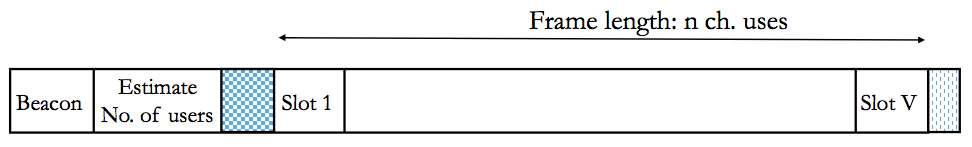
\includegraphics[width=4.5in]{\mac_figpath/slotstructurewithoutfb.png}
%  \begin{tikzpicture}[
  font=\footnotesize,
  >=stealth',
  line width=1pt,
  packet/.style={rectangle, minimum height=4mm, minimum width=14mm, draw=black, fill=gray!10, rounded corners, line width=0.5pt}
]

\draw [->] (0,-0.05) -- (9.75,-0.05);
\draw (0.25,-0.175) -- (0.25,2.95);
\foreach \x in {1,...,5} {
  \draw (1.5*\x+0.25,-0.175) -- (1.5*\x+0.25,0.075);
  \draw[dotted] (1.5*\x+0.25,0.075) -- (1.5*\x+0.25,2.75);
}
\draw (9.25,-0.175) -- (9.25,2.95);
\draw[dashed] (0,2.05) -- (9.5,2.05);
\draw[dashed] (0,2.55) -- (9.5,2.55);

\foreach \x in {1,...,6} {
  \node (t\x) at (1.5*\x-0.5,2.3) {slot~\x};
}
\node (round) at (4.75,2.95) {\textbf{Round}};
\node (start) at (0.25,3.2) {start};
\node (end) at (9.25,3.2) {end};

\node[packet] (p12) at (2.5,0.25) {$w_1$};
\node[packet] (p16) at (8.5,0.25) {$w_1$};
\node[packet] (p21) at (1.0,0.75) {$w_2$};
\node[packet] (p23) at (4.0,0.75) {$w_2$};
\node[packet] (p24) at (5.5,0.75) {$w_2$};
\node[packet] (p31) at (1.0,1.25) {$w_3$};
\node[packet] (p35) at (7.0,1.25) {$w_3$};
\node[packet] (p36) at (8.5,1.25) {$w_3$};
\node[packet] (p42) at (2.5,1.75) {$w_4$};
\node[packet] (p43) at (4.0,1.75) {$w_4$};
\node[packet] (p45) at (7.0,1.75) {$w_4$};

\end{tikzpicture}


\end{frame}

%%%%%%%%%%%%----------------------------------------------------------------------------------%%%%%%%%%%%%%%%
\begin{frame}\frametitle{Problem statement}
  \begin{itemize}
  \setlength{\itemsep}{3pt}
  \item $K$ active users. $K\in[25:300]$
  \item Each user has a $B$-bit message. $B$ is small $\approx 100$
  \item $n$ channel uses available per round. $n=30,000$ 
  \item {\small regime of interest for LP-WAN standards such as LoRaWAN, Weightless}
\end{itemize}
  \pause
  \vspace{2ex}

  \begin{itemize}
  \item $\{w_1,w_2,\ldots,w_K\}$ - set of messages to be transmitted
  \vspace{2.5pt}
  \item Power constraint -$~\frac{1}{n}\mathbb{E}_w[||\xv_w||^2]\leq P$
  \vspace{2.5pt}
  \item Channel model $\yv=\sum_{j=1,\ldots,K}\xv_{w_j}+\zv$. $\vec{z}\sim\mc{N}(0,\mathbf{I}_n)$
  \item If $\mc{L}(\yv)=\{\hat{w}_1,\ldots,\hat{w}_K\}$ is the decoder output, $P_e=\frac{1}{K}\sum\limits_{i=1}^{K} \Pr\left( w_i \notin \mc{L}(\yv) \right) $
  \end{itemize}
      \pause
      \vspace{3ex}
  \begin{block}{Objective}
 Design a coding scheme minimizing the required SNR $P$ such that 
 \begin{itemize}
 \item the encoding and decoding complexities are polynomial in $K,n$ and $B$
 \item prob. of decoding error per user $P_e\leq \epsilon\in [0.05,0.1]$
\end{itemize} 
  \end{block}
 
\end{frame}

%%%%%%%%%%%%----------------------------------------------------------------------------------%%%%%%%%%%%%%%%
\begin{frame} \frametitle{Multiple access - Over the years}
	\begin{itemize} 
	\item {[Polyanskiy 2017]} Gaussian coding for unsourced MAC 
	\vspace{3pt}
	\begin{itemize}	\setlength{\itemsep}{4pt}
		\item Derived achievability limits via random Gaussian coding 
			\begin{itemize}
				\item MMSE decoder: {\color{red} exponential complexity} in $B,K$. $\mc{O}(n\cdot\binom{2^B}{K})\approx\mc{O}(n2^{BK})$
			\end{itemize}
			\item In comparison, ALOHA, TIN found to be very energy-inefficient for $K\gtrapprox100$
	\end{itemize}
	\pause 
		\centering
		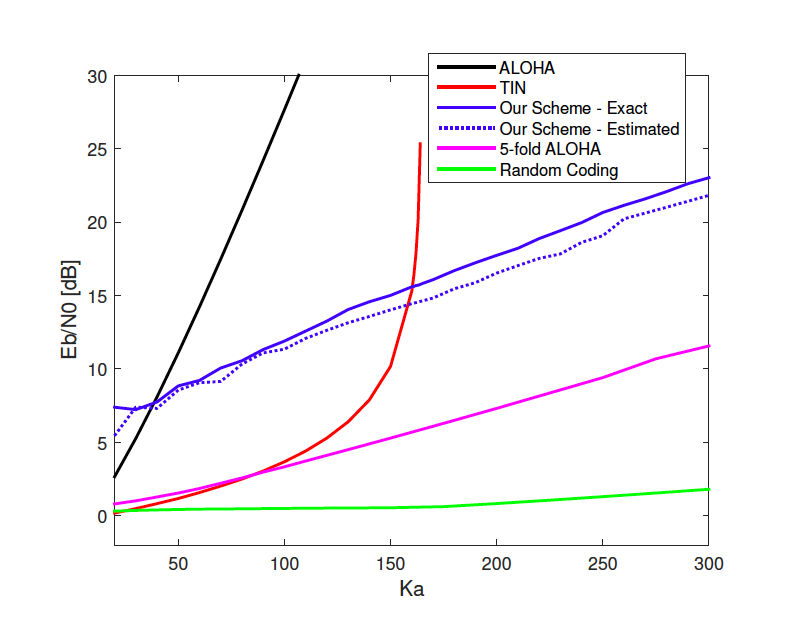
\includegraphics[width=2.8in]{\mac_figpath/OP_2017.png}
\end{itemize}
\end{frame}

%%%%%%%%%%%%----------------------------------------------------------------------------------%%%%%%%%%%%%%%%
\begin{frame}
\begin{itemize}
	\item {[OP-2017]} Low complexity coding scheme for unsourced MAC
	\begin{itemize}\setlength{\itemsep}{4pt}
		\item Concatenated code for $T$-GMAC: Integer forcing and mod-$2$ addition MAC 
		\item {\color{blue} polynomial} encoding and decoding complexity $\mc{O}\left(\max(n, KB^2)\right)$
		\item {\color{blue} outperforms} existing strategies, however {\color{red} $\approx 20dB$ away} from [YP17] ach. limit
		\pause
		\begin{itemize}	\setlength{\itemsep}{2pt}
		\item sub-optimal coding scheme for the $T$-user real adder GMAC
		\item ``capacity achieving low complexity \emph{same-codebook} schemes for the $T$-GMAC channel seems to be a challenging task"
		\item absence of iterative successive interference cancellation(SIC)
		\end{itemize}
	\end{itemize}
\end{itemize}
%	\pause
	\centering
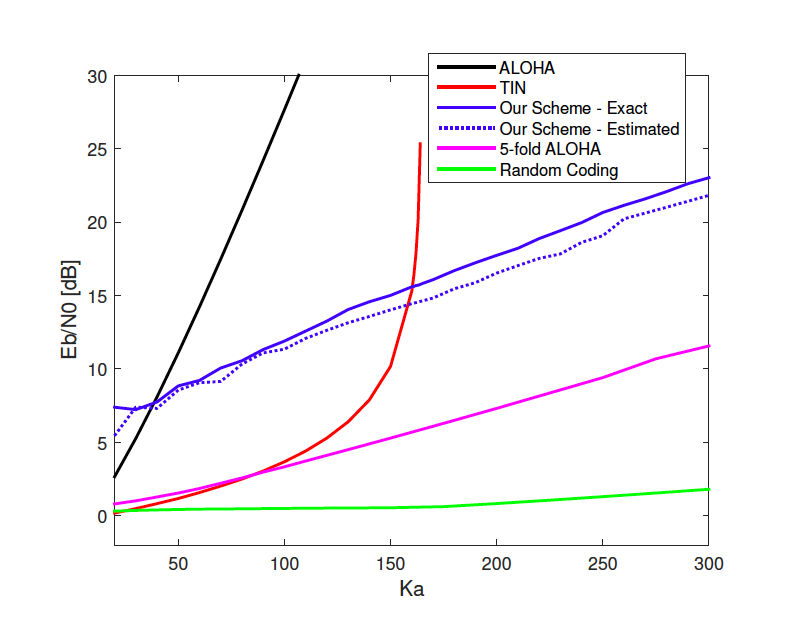
\includegraphics[width=2.4in]{\mac_figpath/OP_2017.png}	
\end{frame}

%%%%%%%%%%%%----------------------------------------------------------------------------------%%%%%%%%%%%%%%%
\begin{frame}\frametitle{Main Result}
\only<1-2>{
%Main features of the proposed scheme:
\begin{itemize}
%\item Same codebook for all the users. Encoder solely depends on the message
%\item Two stages of encoding:
%	\begin{itemize}
%	\setlength{\itemsep}{2pt}
%	\item encoder within a slot: Code with close to optimal performance for $T$-GMAC
%	\item encoder across slots: above codeword is repeated in multiple slots
%    \item repetition pattern is dependent solely on the message
%	\end{itemize}
\item "same-code" design which is close to optimal for $T$-GMAC
\item Peeling based successive interference cancellation(SIC) decoding across slots
\end{itemize}
}
\only<3>{
\centering
\resizebox{0.55\textwidth}{!}{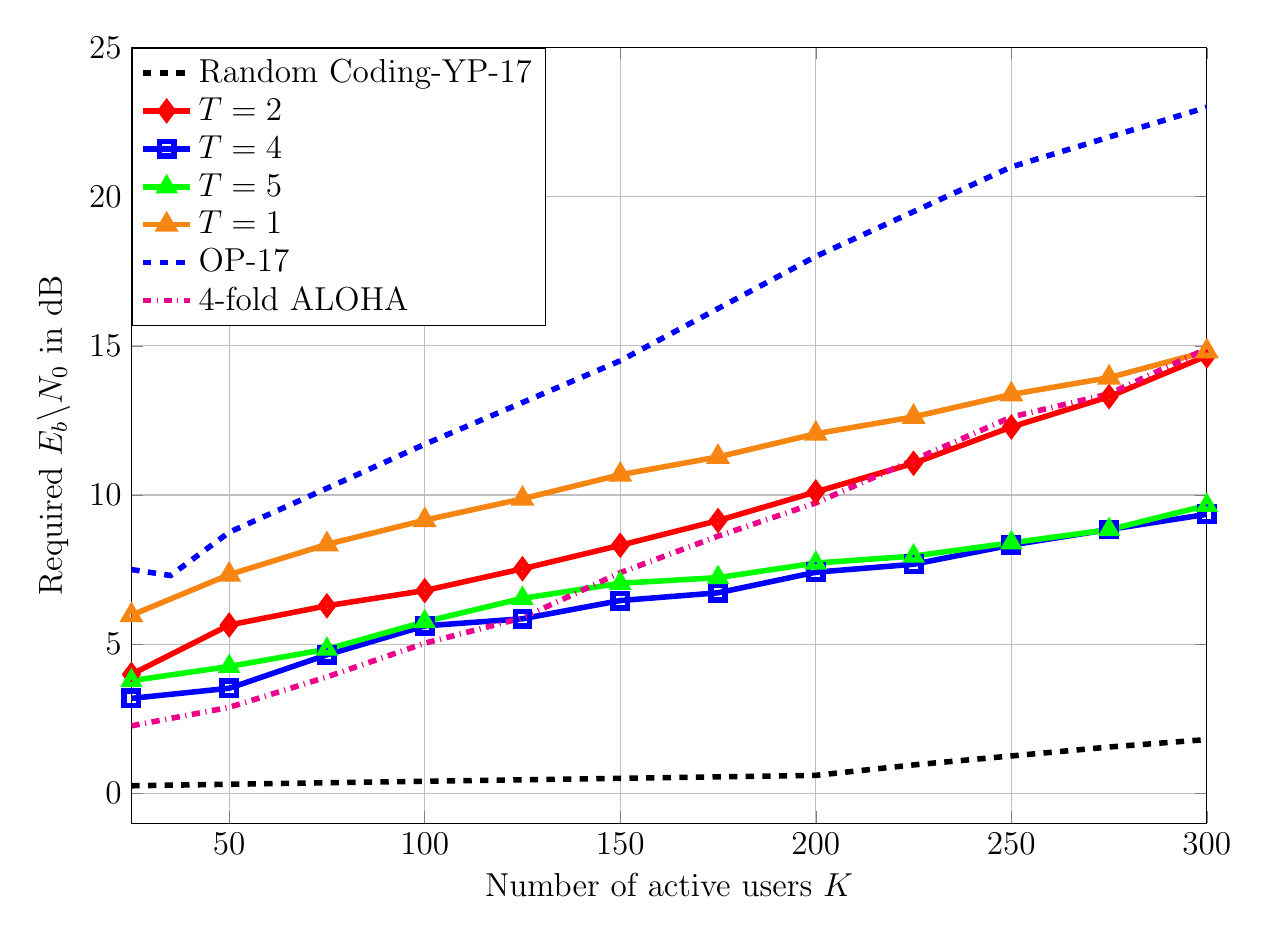
\begin{tikzpicture}
\def\fsize{\large}

\pgfplotsset{every y tick label/.append style={font=\fsize}}
\pgfplotsset{every x tick label/.append style={font=\fsize}}

\begin{axis}[%
width=6in,
height=4.5in,
xmin=25,
xmax=300,
xtick = {50,100,...,300},
xlabel={\fsize{Number of active users $K$}},
ylabel={\fsize{Required $E_b\backslash N_0$ in dB}},
xmajorgrids,
xminorgrids,
ymin=-1,
ymax=25,
ytick = {-5,0,...,30},
yminorticks=true,
ymajorgrids,
yminorgrids,
legend style={at={(0,1)},anchor=north west, draw=black,fill=white,legend cell align=left,font=\fsize}
]

\addplot [color=black,solid,dashed, line width=2.0pt]
  table[row sep=crcr]{
  25     0.25\\
 50     0.3\\
 75     0.35\\
100     0.4\\
125     0.45\\
150     0.5\\
175    0.55\\
200  0.60\\
225 0.95\\
250 1.25\\
275 1.55\\
300 1.8\\
};
\addlegendentry{Random Coding-YP-17};

\addplot [color=red,solid,mark=diamond,mark size=3.0, line width=2.0pt]
  table[row sep=crcr]{
  25   3.9849  \\
  50   5.6396\\
  75   6.2855  \\
100  6.7952 \\
125  7.5262 \\
150  8.3122 \\
175  9.1418 \\
200  10.103 \\
225  11.062 \\
250  12.279 \\
275 13.296 \\
300 14.6648 \\
};
\addlegendentry{$T=2$};

\addplot [color=blue,solid,mark=square,mark size=2.6, line width=2.0pt]
  table[row sep=crcr]{
 25 3.18\\
 50 3.52\\
 75 4.64\\
100 5.61\\
125 5.85\\
150 6.46\\
175 6.72\\
200 7.41\\
 225 7.6772\\
 250 8.3217\\
 275 8.8428\\
 300 9.3520 \\
};
\addlegendentry{$T=4$};

%\addplot [color=blue,dotted, line width=2.0pt]
%  table[row sep=crcr]{
% 25 2.8815\\
% 50 3.2015\\
% 75 4.3960\\
%100 5.30\\
%125 5.5533\\
%150 6.1838\\
%175 6.4562\\
%200 7.1900\\
% 225 7.4664\\
% 250 8.1394\\
% 275 8.6810\\
% 300 9.2079 \\
%};
%\addlegendentry{$T=4$,ML-CS};

\addplot [color=green,mark=triangle,mark size=2.7, line width=2.0pt]
  table[row sep=crcr]{
 25 3.7732\\
 50 4.25\\
 75 4.8287\\
100 5.7503\\
125 6.5344\\
150 7.0391\\
175 7.2288\\
200 7.7171\\
 225 7.9514 \\
250 8.3968\\
275 8.8358\\
300  9.6524\\
};
\addlegendentry{$T=5$};

\addplot [color=BurntOrange,solid,mark=triangle,mark size=3.0, line width=2.0pt]
table[row sep=crcr]{
25 5.9675\\
50 7.33\\
75 8.3433\\
100 9.1555\\
125 9.8708\\
150 10.679\\
175 11.275\\
200 12.052 \\
225 12.61860 \\
250 13.3702 \\
275 13.934\\
300 14.816\\
 };
\addlegendentry{$T=1$}; %After Yury's correction



\addplot [color=blue,dashed, line width=2.0pt]
  table[row sep=crcr]{
  25   7.50 \\
   35   7.30 \\
  50   8.75 \\
  100 11.7 \\
  150 14.50\\
%175  6.7814 \\
200  18\\
%225  7.6838 \\
250  21\\
%275  8.4960 \\
300 23\\
};
\addlegendentry{OP-17};

\addplot [color=magenta,dash dot,line width=2.0pt]
  table[row sep=crcr]{
  25   2.26  \\
  50   2.88  \\
  75   3.90  \\
 100   5.03 \\
  125.0000    5.8798 \\
  150.0000    7.3954 \\
  175.0000    8.6199 \\
  200.0000    9.7328 \\
  225.0000   11.1761\\
  250.0000   12.6127\\
  275.0000   13.3907\\
  300.0000   14.9116\\
  };
\addlegendentry{4-fold ALOHA};

\end{axis}
\end{tikzpicture}}
}
%\item Message is split into two parts: $w=(w^{\mathrm{p}},w^{\mathrm{c}})$
%\pause
%	\begin{itemize}
%	\item $w^{\mathrm{c}}$: encoded using an LDPC type channel code
%	\item Designed for a $T$-user Gaussian multiple access(GMAC) channel
%\pause
%	\item $w^{\mathrm{p}}$: preamble, chooses an interleaver for the channel code
%	\item  preamble encoded using a compressed sensing type scheme
%	\end{itemize}
%\item Encoded codeword is repeated in multiple slots
%	\begin{itemize}
%	\item  repetition pattern is dependent solely on the message $w$
%	\end{itemize}
%	\pause
\onslide<2-3>{
\begin{block}{Main result}
	\begin{itemize}
		\item Polynomial encoding and decoding complexity: $\mc{O}(KT^6+Kn)\approx \mc{O}\left(nK)\right)$
		\item {\color{blue} Best among the existing coding strategies} with poly. complexity
		\item Overall coding scheme outperforms [OP-2017] by $\approx 13$dB
		\item Only $6$dB away from the Gaussian random coding limit.
	 	\item ``same code" design for $T$-user GMAC that is $\approx 2$dB away from FBL limit
\end{itemize} 
\end{block}
}
\end{frame}
%%%%%%%%%%%%----------------------------------------------------------------------------------%%%%%%%%%%%%%%%
\subsection{Communication scheme}
\begin{frame}
\frametitle{Proposed coding scheme}
\centering
\resizebox{0.85\textwidth}{!}{\begin{tikzpicture}

\def\nodewidth{0.5in}
\def\fsize{\Large}
\def\sfsize{\normalsize}
\def\xoffs{0.5in}
\def\ya{3.5}
\def\xr{4}
\def\xslots{11}
\def\xdec{18}
\tikzstyle{block} = [rectangle, draw, thick, opacity=0.7,line width =2, minimum size=\nodewidth]
\tikzstyle{vertRectangle} = [rectangle, draw, opacity=0.7,line width =2, minimum width=\nodewidth, minimum height=12*\nodewidth]
\tikzstyle{opnode} = [rectangle, draw, thick,opacity=0.7,line width=1, minimum size=0.2in]

\node[block] (r11) at (-0.5,0){\fsize \textbf{Encoder} $\mc{C}$};
\node[block] (r21) at (\xr,0) {\fsize \begin{tabular}{c}
Repeat \\
$\ell_{w_1}$ times
\end{tabular}};

\node[block] (r12) at (-0.5,-\ya){\fsize \textbf{Encoder} $\mc{C}$};
\node[block] (r22) at (\xr,-\ya) {\fsize \begin{tabular}{c}
Repeat \\
$\ell_{w_i}$ times
\end{tabular}};

\node[block] (r13) at (-0.5,-3*\ya){\fsize \textbf{Encoder} $\mc{C}$};
\node[block] (r23) at (\xr,-3*\ya) {\fsize 
\begin{tabular}{c}
Repeat \\
$\ell_{w_{K_a}}$ times
\end{tabular}};

\node[vertRectangle] (r3) at (\xslots,-1.5*\ya){\fsize \bf Slots};
\node[vertRectangle,align=center] (r4) at (\xdec,-1.5*\ya){\fsize \bf \begin{tabular}{c}
Up to T-users\\
jointly decoded \\ 
 in each slot\\
+ \\ 
Successive Interference \\
Cancellation (SIC) \\
across slots.
\end{tabular}
};

\draw[<-, thick, line width=2] (r11.west)--node[midway, above]{\fsize $w_1$}+(-\xoffs,0);
\draw[->, thick, line width=2] (r11.east)--node[midway, above]{\fsize $\xv_{w_1}$}(r21.west);

\draw[<-, thick, line width=2] (r12.west)--node[midway, above]{\fsize $w_i$}+(-\xoffs,0);
\draw[->, thick, line width=2] (r12.east)--node[midway, above]{\fsize $\xv_{w_i}$}(r22.west);

\draw[<-, thick, line width=2] (r13.west)--node[midway, above]{\fsize $w_{K_a}$}+(-\xoffs,0);
\draw[->, thick, line width=2] (r13.east)--node[midway, above]{\fsize $\xv_{w_{K_a}}$}(r23.west);

\draw[transform canvas={yshift=-\nodewidth},thick] (r3.north west) -- (r3.north east);
\draw[transform canvas={yshift=-2*\nodewidth},thick] (r3.north west) -- (r3.north east);
\draw[transform canvas={yshift=-3*\nodewidth},thick] (r3.north west) -- (r3.north east);
\draw[transform canvas={yshift=\nodewidth}] (r3.south west) -- (r3.south east);
\node [below=0.3*\nodewidth of r3.north](s1) {\fsize Slot 1};
\node [below=1.3*\nodewidth of r3.north](s2) {\fsize Slot 2};
\node [below=2.3*\nodewidth of r3.north](s3) {\fsize Slot 3};
\node [above=0.3*\nodewidth of r3.south](s4) {\fsize Slot V};
\node [below=3.5*\nodewidth of r3.north]() {\Huge $\vdots$};
\node [above=3.5*\nodewidth of r3.south]() {\Huge $\vdots$};


\begin{scope}[very thick,decoration={
    markings,
    mark=at position 0.5 with {\arrow{>}}}
    ] 
\draw[transform canvas={yshift=-0.5*\nodewidth},postaction={decorate}] (r3.north east) -- (r4.north west);
\draw[transform canvas={yshift=-1.5*\nodewidth},postaction={decorate}] (r3.north east) -- (r4.north west);
\draw[transform canvas={yshift=-2.5*\nodewidth},postaction={decorate}] (r3.north east) -- (r4.north west);
\draw[transform canvas={yshift=0.5*\nodewidth},postaction={decorate}] (r3.south east) -- (r4.south west);
\end{scope}

\draw[<-, thick] (r3.north west)++(0,-2.5*\nodewidth)--(r21.east);
\draw[<-, thick] (r3.north west)++(0,-9.5*\nodewidth)--(r21.east);
\path (r21.east) -- ++(5:0.5cm) coordinate(r21a) 
		  (r21.east) -- ++(320:0.5cm) coordinate(r21b) ;
%\draw[<->,thick] (r21a) to [bend left=30] (r21b) node [right] {\fsize $L_{w_1}$};

\draw[<-, thick] (r3.north west)++(0,-2.5*\nodewidth)--(r22.east);
\draw[<-, thick] (r3.north west)++(0,-1.5*\nodewidth)--(r22.east);
\draw[<-, thick] (r3.north west)++(0,-8.5*\nodewidth)--(r22.east);
\path (r22.east) -- ++(25:0.5cm) coordinate(r22a) 
		  (r22.east) -- ++(335:0.5cm) coordinate(r22b) ;
%\draw[<->,thick] (r22a) to [bend left=30] (r22b) node [right] {\fsize $L_{w_i}$};


\draw[<-, thick] (r3.north west)++(0,-0.5*\nodewidth)--(r23.east);
\draw[<-, thick] (r3.north west)++(0,-6.5*\nodewidth)--(r23.east);
\path (r23.east) -- ++(22:0.5cm) coordinate(r23a) 
		  (r23.east) -- ++(55:0.5cm) coordinate(r23b) ;
%\draw[<->] (r23a) to [bend right=30] (r23b) node [right] {\fsize $L_{w_{K_a}}$};


\draw[->, thick, line width=2] (r4.east)--node[midway, above]{\fsize $\widehat{w}_1,\ldots, \widehat{w}_{K_a}$}+(2.5*\xoffs,0);
\end{tikzpicture}}
%\begin{itemize}
%\end{itemize}

\end{frame}



%%%%%%%%%%%%----------------------------------------------------------------------------------%%%%%%%%%%%%%%%
\begin{frame}
\frametitle{Encoder within a slot}
\only<1>{
	\begin{itemize}
	\item B-bit message $w=(\wpdash,\wc).$ $\wpdash\in[1:2^{B_{\mathrm{p}}}],\wc\in[1:2^{B_{\mathrm{c}}}]$
		\begin{itemize}
			\item $B_{\mathrm{p}} \ll B_{\mathrm{c}}$ and $ B=B_{\mathrm{c}}+B_{\mathrm{p}}$
			\item $\wpdash,\wc$ encoded by compressed sensing and channel coding parts resp.
		\end{itemize}
	\end{itemize}
	\centering
\resizebox{0.8\textwidth}{!}{\begin{tikzpicture}

\def\nodewidth{0.5in}
\def\fsize{\Large}
\def\sfsize{\normalsize}
\def\xoffs{0.5in}
\def\ya{3.5}
\def\xr{4}
\def\xslots{11}
\def\xdec{18}
\tikzstyle{block} = [rectangle, draw, thick, opacity=0.7,line width =2, minimum size=\nodewidth]
\tikzstyle{vertRectangle} = [rectangle, draw, opacity=0.7,line width =2, minimum width=\nodewidth, minimum height=12*\nodewidth]
\tikzstyle{opnode} = [rectangle, draw, thick,opacity=0.7,line width=1, minimum size=0.2in]

\node[block] (r11) at (-0.5,0){\fsize \textbf{Encoder} $\mc{C}$};
\node[block] (r21) at (\xr,0) {\fsize \begin{tabular}{c}
Repeat \\
$\ell_{w_1}$ times
\end{tabular}};

\node[block] (r12) at (-0.5,-\ya){\fsize \textbf{Encoder} $\mc{C}$};
\node[block] (r22) at (\xr,-\ya) {\fsize \begin{tabular}{c}
Repeat \\
$\ell_{w_i}$ times
\end{tabular}};

\node[block] (r13) at (-0.5,-3*\ya){\fsize \textbf{Encoder} $\mc{C}$};
\node[block] (r23) at (\xr,-3*\ya) {\fsize 
\begin{tabular}{c}
Repeat \\
$\ell_{w_{K_a}}$ times
\end{tabular}};

\node[vertRectangle] (r3) at (\xslots,-1.5*\ya){\fsize \bf Slots};
\node[vertRectangle,align=center] (r4) at (\xdec,-1.5*\ya){\fsize \bf \begin{tabular}{c}
Up to T-users\\
jointly decoded \\ 
 in each slot\\
+ \\ 
Successive Interference \\
Cancellation (SIC) \\
across slots.
\end{tabular}
};

\draw[<-, thick, line width=2] (r11.west)--node[midway, above]{\fsize $w_1$}+(-\xoffs,0);
\draw[->, thick, line width=2] (r11.east)--node[midway, above]{\fsize $\xv_{w_1}$}(r21.west);

\draw[<-, thick, line width=2] (r12.west)--node[midway, above]{\fsize $w_i$}+(-\xoffs,0);
\draw[->, thick, line width=2] (r12.east)--node[midway, above]{\fsize $\xv_{w_i}$}(r22.west);

\draw[<-, thick, line width=2] (r13.west)--node[midway, above]{\fsize $w_{K_a}$}+(-\xoffs,0);
\draw[->, thick, line width=2] (r13.east)--node[midway, above]{\fsize $\xv_{w_{K_a}}$}(r23.west);

\draw[transform canvas={yshift=-\nodewidth},thick] (r3.north west) -- (r3.north east);
\draw[transform canvas={yshift=-2*\nodewidth},thick] (r3.north west) -- (r3.north east);
\draw[transform canvas={yshift=-3*\nodewidth},thick] (r3.north west) -- (r3.north east);
\draw[transform canvas={yshift=\nodewidth}] (r3.south west) -- (r3.south east);
\node [below=0.3*\nodewidth of r3.north](s1) {\fsize Slot 1};
\node [below=1.3*\nodewidth of r3.north](s2) {\fsize Slot 2};
\node [below=2.3*\nodewidth of r3.north](s3) {\fsize Slot 3};
\node [above=0.3*\nodewidth of r3.south](s4) {\fsize Slot V};
\node [below=3.5*\nodewidth of r3.north]() {\Huge $\vdots$};
\node [above=3.5*\nodewidth of r3.south]() {\Huge $\vdots$};


\begin{scope}[very thick,decoration={
    markings,
    mark=at position 0.5 with {\arrow{>}}}
    ] 
\draw[transform canvas={yshift=-0.5*\nodewidth},postaction={decorate}] (r3.north east) -- (r4.north west);
\draw[transform canvas={yshift=-1.5*\nodewidth},postaction={decorate}] (r3.north east) -- (r4.north west);
\draw[transform canvas={yshift=-2.5*\nodewidth},postaction={decorate}] (r3.north east) -- (r4.north west);
\draw[transform canvas={yshift=0.5*\nodewidth},postaction={decorate}] (r3.south east) -- (r4.south west);
\end{scope}

\draw[<-, thick] (r3.north west)++(0,-2.5*\nodewidth)--(r21.east);
\draw[<-, thick] (r3.north west)++(0,-9.5*\nodewidth)--(r21.east);
\path (r21.east) -- ++(5:0.5cm) coordinate(r21a) 
		  (r21.east) -- ++(320:0.5cm) coordinate(r21b) ;
%\draw[<->,thick] (r21a) to [bend left=30] (r21b) node [right] {\fsize $L_{w_1}$};

\draw[<-, thick] (r3.north west)++(0,-2.5*\nodewidth)--(r22.east);
\draw[<-, thick] (r3.north west)++(0,-1.5*\nodewidth)--(r22.east);
\draw[<-, thick] (r3.north west)++(0,-8.5*\nodewidth)--(r22.east);
\path (r22.east) -- ++(25:0.5cm) coordinate(r22a) 
		  (r22.east) -- ++(335:0.5cm) coordinate(r22b) ;
%\draw[<->,thick] (r22a) to [bend left=30] (r22b) node [right] {\fsize $L_{w_i}$};


\draw[<-, thick] (r3.north west)++(0,-0.5*\nodewidth)--(r23.east);
\draw[<-, thick] (r3.north west)++(0,-6.5*\nodewidth)--(r23.east);
\path (r23.east) -- ++(22:0.5cm) coordinate(r23a) 
		  (r23.east) -- ++(55:0.5cm) coordinate(r23b) ;
%\draw[<->] (r23a) to [bend right=30] (r23b) node [right] {\fsize $L_{w_{K_a}}$};


\draw[->, thick, line width=2] (r4.east)--node[midway, above]{\fsize $\widehat{w}_1,\ldots, \widehat{w}_{K_a}$}+(2.5*\xoffs,0);
\end{tikzpicture}}	
	}
	\only<2->{
	\begin{itemize}
	\item B-bit message $w=(\wpdash,\wc).$ $\wpdash\in[1:2^{B_{\mathrm{p}}}],\wc\in[1:2^{B_{\mathrm{c}}}]$
	\begin{itemize}
		\item $B_{\mathrm{p}} \ll B_{\mathrm{c}}$ and $ B=B_{\mathrm{c}}+B_{\mathrm{p}}$
		\item $\wpdash,\wc$ encoded by compressed sensing and channel coding parts resp.
	\end{itemize}
	\item Compressed sensing encoder ($\wpdash$)
	\begin{itemize}
		\item sensing matrix $\mathbf{A}=[\av_1,\av_2,\ldots,\av_{2^{B_{\mathrm{p}}}}]$
		\end{itemize}
	\item Channel coding component ($\wc$)
	\begin{itemize}
		\item  $\mc{C}_{\mathrm{c}}=[\cv_1,\cv_2,\ldots,\cv_{2^{B_{\mathrm{c}}}}]$ be a LDPC type channel code
		\item interleaver $\pi_{f(\wpdash)}$ such that $f(\wpdash)\in [1:N_{\mathrm{c}}!]$
		\end{itemize}
\end{itemize}
\vspace{3ex}
\centering
\resizebox{0.6\textwidth}{!}{\begin{tikzpicture}

\def\fsize{\normalsize}
\def\fsizes{\scriptsize}
\def\ext{1}
%Message node and final codeword Rectangle
\node[font=\fsize,draw,rectangle] (msg) at (3,1) {\fsizes $w=(\wpdash,\wc)$};
\node[rectangle, draw, minimum width=2.7in,thick] (codeword) at (3+0.5\ext,1+2*\ext) {\fsizes $\pi_{f(\wpdash)}(\vec{c}_{\wc})$};
%$c_{w}(\pi_{\tau_{\wpdash}^1}),c_{w}(\pi_{\tau_{\wpdash}^2}),\ldots,c_{w}(\pi_{\tau_{\wpdash}})$};


% From messages to Ch. Encoder and Compressive Sensing Encoder
\draw [->] (msg.east) -- +(0:\ext) node[midway, above] {\fsizes $\wc$} node[draw, inner sep=5pt,at end, anchor= west] (encoder) {\fsizes Ch. Encoder} ;
\draw [->] (msg.west) -- +(0:-\ext) node[midway, above] {\fsizes  $\wpdash$} node[draw, inner sep=5pt,at end, anchor= east] (CSencoder) {\fsizes $\mathbf{A}$}; %{Sensing Matrix $\mathbf{A}$};

%From Encoder to north
\path (encoder.north)-- +(90:0.6*\ext) node[draw, rectangle,fill=white](CWperm){\fsizes Permute};
\draw[->] (encoder.north)-- (CWperm.south) node[midway,right]{\fsizes $\cv_{\wc}$};
\draw[->](CWperm.north)-- (CWperm.north |- codeword.south) node[midway, right]{\fsizes $\pi_{f(\wpdash)}(\cv_{\wc})$};

%From CSEncoder to north
\draw[->](CSencoder.north)-- (CSencoder.north |- codeword.south) node[midway, left]{\fsizes  $\av^T_{\wpdash}$};

%Partitioning the Tx codeword block
\path let \p{A}=(codeword) in (3-1.7*\ext,\y{A})node (partition){} -- (partition |- codeword.north);
\draw (partition |- codeword.north) -- (partition |- codeword.south) ;
\node () at (partition -| CSencoder) {\fsizes $\av_{\wpdash}$};
\node [right] at (codeword.east) {$\cv_{w}$};

\draw [->] (msg.north) -- (msg.north |- CWperm.west)node[midway,left]{\fsizes $\wpdash$} -- (CWperm.west) node[midway,above] {\fsizes $f(\wpdash)$};
\end{tikzpicture} }
}
\end{frame}

%%%%%%%%%%%%----------------------------------------------------------------------------------%%%%%%%%%%%%%%%
\begin{frame}
\frametitle{Encoding across slots}
\begin{itemize}
	\item Encoder within a slot: $w=(\wpdash,\wc)\rightarrow \vec{x}_w,~\frac{1}{N}||\vec{x}_w||^2=P_{\text{slot}}$
	\item Each user 
	\begin{itemize}
		\item chooses a repetition parameter $\ell_{w}=g(w), g:[1:M] \rightarrow [1:V]$ 
		\item chooses $\ell_{w}$ slots from $[1:V]$ acc. to $h(w)$ and repeats in those slots
	\end{itemize}
	\onslide<2->{
 	\item Left d.d is determined by the function $g$
	\begin{itemize}
		\item  $g_{\beta}(\cdot)$ chosen such that $L(x)=\beta x+(1-\beta)x^2$ is the left d.d
		\item $P=(2-\beta)P_{\text{slot}}$
	\end{itemize}
	}
\end{itemize}
%\vspace{1ex}
	\centering
\resizebox{0.7\textwidth}{!}{\begin{tikzpicture}

\def\nodewidth{0.5in}
\def\fsize{\Large}
\def\sfsize{\normalsize}
\def\xoffs{0.5in}
\def\ya{3.5}
\def\xr{4}
\def\xslots{11}
\def\xdec{18}
\tikzstyle{block} = [rectangle, draw, thick, opacity=0.7,line width =2, minimum size=\nodewidth]
\tikzstyle{vertRectangle} = [rectangle, draw, opacity=0.7,line width =2, minimum width=\nodewidth, minimum height=12*\nodewidth]
\tikzstyle{opnode} = [rectangle, draw, thick,opacity=0.7,line width=1, minimum size=0.2in]

\node[block] (r11) at (-0.5,0){\fsize \textbf{Encoder} $\mc{C}$};
\node[block] (r21) at (\xr,0) {\fsize \begin{tabular}{c}
Repeat \\
$\ell_{w_1}$ times
\end{tabular}};

\node[block] (r12) at (-0.5,-\ya){\fsize \textbf{Encoder} $\mc{C}$};
\node[block] (r22) at (\xr,-\ya) {\fsize \begin{tabular}{c}
Repeat \\
$\ell_{w_i}$ times
\end{tabular}};

\node[block] (r13) at (-0.5,-3*\ya){\fsize \textbf{Encoder} $\mc{C}$};
\node[block] (r23) at (\xr,-3*\ya) {\fsize 
\begin{tabular}{c}
Repeat \\
$\ell_{w_{K_a}}$ times
\end{tabular}};

\node[vertRectangle] (r3) at (\xslots,-1.5*\ya){\fsize \bf Slots};
\node[vertRectangle,align=center] (r4) at (\xdec,-1.5*\ya){\fsize \bf \begin{tabular}{c}
Up to T-users\\
jointly decoded \\ 
 in each slot\\
+ \\ 
Successive Interference \\
Cancellation (SIC) \\
across slots.
\end{tabular}
};

\draw[<-, thick, line width=2] (r11.west)--node[midway, above]{\fsize $w_1$}+(-\xoffs,0);
\draw[->, thick, line width=2] (r11.east)--node[midway, above]{\fsize $\xv_{w_1}$}(r21.west);

\draw[<-, thick, line width=2] (r12.west)--node[midway, above]{\fsize $w_i$}+(-\xoffs,0);
\draw[->, thick, line width=2] (r12.east)--node[midway, above]{\fsize $\xv_{w_i}$}(r22.west);

\draw[<-, thick, line width=2] (r13.west)--node[midway, above]{\fsize $w_{K_a}$}+(-\xoffs,0);
\draw[->, thick, line width=2] (r13.east)--node[midway, above]{\fsize $\xv_{w_{K_a}}$}(r23.west);

\draw[transform canvas={yshift=-\nodewidth},thick] (r3.north west) -- (r3.north east);
\draw[transform canvas={yshift=-2*\nodewidth},thick] (r3.north west) -- (r3.north east);
\draw[transform canvas={yshift=-3*\nodewidth},thick] (r3.north west) -- (r3.north east);
\draw[transform canvas={yshift=\nodewidth}] (r3.south west) -- (r3.south east);
\node [below=0.3*\nodewidth of r3.north](s1) {\fsize Slot 1};
\node [below=1.3*\nodewidth of r3.north](s2) {\fsize Slot 2};
\node [below=2.3*\nodewidth of r3.north](s3) {\fsize Slot 3};
\node [above=0.3*\nodewidth of r3.south](s4) {\fsize Slot V};
\node [below=3.5*\nodewidth of r3.north]() {\Huge $\vdots$};
\node [above=3.5*\nodewidth of r3.south]() {\Huge $\vdots$};


\begin{scope}[very thick,decoration={
    markings,
    mark=at position 0.5 with {\arrow{>}}}
    ] 
\draw[transform canvas={yshift=-0.5*\nodewidth},postaction={decorate}] (r3.north east) -- (r4.north west);
\draw[transform canvas={yshift=-1.5*\nodewidth},postaction={decorate}] (r3.north east) -- (r4.north west);
\draw[transform canvas={yshift=-2.5*\nodewidth},postaction={decorate}] (r3.north east) -- (r4.north west);
\draw[transform canvas={yshift=0.5*\nodewidth},postaction={decorate}] (r3.south east) -- (r4.south west);
\end{scope}

\draw[<-, thick] (r3.north west)++(0,-2.5*\nodewidth)--(r21.east);
\draw[<-, thick] (r3.north west)++(0,-9.5*\nodewidth)--(r21.east);
\path (r21.east) -- ++(5:0.5cm) coordinate(r21a) 
		  (r21.east) -- ++(320:0.5cm) coordinate(r21b) ;
%\draw[<->,thick] (r21a) to [bend left=30] (r21b) node [right] {\fsize $L_{w_1}$};

\draw[<-, thick] (r3.north west)++(0,-2.5*\nodewidth)--(r22.east);
\draw[<-, thick] (r3.north west)++(0,-1.5*\nodewidth)--(r22.east);
\draw[<-, thick] (r3.north west)++(0,-8.5*\nodewidth)--(r22.east);
\path (r22.east) -- ++(25:0.5cm) coordinate(r22a) 
		  (r22.east) -- ++(335:0.5cm) coordinate(r22b) ;
%\draw[<->,thick] (r22a) to [bend left=30] (r22b) node [right] {\fsize $L_{w_i}$};


\draw[<-, thick] (r3.north west)++(0,-0.5*\nodewidth)--(r23.east);
\draw[<-, thick] (r3.north west)++(0,-6.5*\nodewidth)--(r23.east);
\path (r23.east) -- ++(22:0.5cm) coordinate(r23a) 
		  (r23.east) -- ++(55:0.5cm) coordinate(r23b) ;
%\draw[<->] (r23a) to [bend right=30] (r23b) node [right] {\fsize $L_{w_{K_a}}$};


\draw[->, thick, line width=2] (r4.east)--node[midway, above]{\fsize $\widehat{w}_1,\ldots, \widehat{w}_{K_a}$}+(2.5*\xoffs,0);
\end{tikzpicture}}	
\end{frame}


%%%%%%%%%%%%----------------------------------------------------------------------------------%%%%%%%%%%%%%%%
\begin{frame}
\frametitle{Decoder}
\begin{itemize}
\item At each slot: Decoder for $T$-user GMAC
	\begin{itemize}
	\item Energy test to estimate the number of users transmitting
	\[
	\hat{R}_{j}= \left[\frac{||\yv_j||^2-N\sigma^2}{P_{\text{slot}}}\right]
	\]
	\item If $	\hat{R}_{j}\leq T$ perform $T$-GMAC decoder in $j$-th slot 
	\end{itemize}
\item Decoder across slots via peeling decoder (SIC)
\end{itemize}
\vspace{2ex}
\centering
\resizebox{0.7\textwidth}{!}{\begin{tikzpicture}

\def\nodewidth{0.5in}
\def\fsize{\Large}
\def\sfsize{\normalsize}
\def\xoffs{0.5in}
\def\ya{3.5}
\def\xr{4}
\def\xslots{11}
\def\xdec{18}
\tikzstyle{block} = [rectangle, draw, thick, opacity=0.7,line width =2, minimum size=\nodewidth]
\tikzstyle{vertRectangle} = [rectangle, draw, opacity=0.7,line width =2, minimum width=\nodewidth, minimum height=12*\nodewidth]
\tikzstyle{opnode} = [rectangle, draw, thick,opacity=0.7,line width=1, minimum size=0.2in]

\node[block] (r11) at (-0.5,0){\fsize \textbf{Encoder} $\mc{C}$};
\node[block] (r21) at (\xr,0) {\fsize \begin{tabular}{c}
Repeat \\
$\ell_{w_1}$ times
\end{tabular}};

\node[block] (r12) at (-0.5,-\ya){\fsize \textbf{Encoder} $\mc{C}$};
\node[block] (r22) at (\xr,-\ya) {\fsize \begin{tabular}{c}
Repeat \\
$\ell_{w_i}$ times
\end{tabular}};

\node[block] (r13) at (-0.5,-3*\ya){\fsize \textbf{Encoder} $\mc{C}$};
\node[block] (r23) at (\xr,-3*\ya) {\fsize 
\begin{tabular}{c}
Repeat \\
$\ell_{w_{K_a}}$ times
\end{tabular}};

\node[vertRectangle] (r3) at (\xslots,-1.5*\ya){\fsize \bf Slots};
\node[vertRectangle,align=center] (r4) at (\xdec,-1.5*\ya){\fsize \bf \begin{tabular}{c}
Up to T-users\\
jointly decoded \\ 
 in each slot\\
+ \\ 
Successive Interference \\
Cancellation (SIC) \\
across slots.
\end{tabular}
};

\draw[<-, thick, line width=2] (r11.west)--node[midway, above]{\fsize $w_1$}+(-\xoffs,0);
\draw[->, thick, line width=2] (r11.east)--node[midway, above]{\fsize $\xv_{w_1}$}(r21.west);

\draw[<-, thick, line width=2] (r12.west)--node[midway, above]{\fsize $w_i$}+(-\xoffs,0);
\draw[->, thick, line width=2] (r12.east)--node[midway, above]{\fsize $\xv_{w_i}$}(r22.west);

\draw[<-, thick, line width=2] (r13.west)--node[midway, above]{\fsize $w_{K_a}$}+(-\xoffs,0);
\draw[->, thick, line width=2] (r13.east)--node[midway, above]{\fsize $\xv_{w_{K_a}}$}(r23.west);

\draw[transform canvas={yshift=-\nodewidth},thick] (r3.north west) -- (r3.north east);
\draw[transform canvas={yshift=-2*\nodewidth},thick] (r3.north west) -- (r3.north east);
\draw[transform canvas={yshift=-3*\nodewidth},thick] (r3.north west) -- (r3.north east);
\draw[transform canvas={yshift=\nodewidth}] (r3.south west) -- (r3.south east);
\node [below=0.3*\nodewidth of r3.north](s1) {\fsize Slot 1};
\node [below=1.3*\nodewidth of r3.north](s2) {\fsize Slot 2};
\node [below=2.3*\nodewidth of r3.north](s3) {\fsize Slot 3};
\node [above=0.3*\nodewidth of r3.south](s4) {\fsize Slot V};
\node [below=3.5*\nodewidth of r3.north]() {\Huge $\vdots$};
\node [above=3.5*\nodewidth of r3.south]() {\Huge $\vdots$};


\begin{scope}[very thick,decoration={
    markings,
    mark=at position 0.5 with {\arrow{>}}}
    ] 
\draw[transform canvas={yshift=-0.5*\nodewidth},postaction={decorate}] (r3.north east) -- (r4.north west);
\draw[transform canvas={yshift=-1.5*\nodewidth},postaction={decorate}] (r3.north east) -- (r4.north west);
\draw[transform canvas={yshift=-2.5*\nodewidth},postaction={decorate}] (r3.north east) -- (r4.north west);
\draw[transform canvas={yshift=0.5*\nodewidth},postaction={decorate}] (r3.south east) -- (r4.south west);
\end{scope}

\draw[<-, thick] (r3.north west)++(0,-2.5*\nodewidth)--(r21.east);
\draw[<-, thick] (r3.north west)++(0,-9.5*\nodewidth)--(r21.east);
\path (r21.east) -- ++(5:0.5cm) coordinate(r21a) 
		  (r21.east) -- ++(320:0.5cm) coordinate(r21b) ;
%\draw[<->,thick] (r21a) to [bend left=30] (r21b) node [right] {\fsize $L_{w_1}$};

\draw[<-, thick] (r3.north west)++(0,-2.5*\nodewidth)--(r22.east);
\draw[<-, thick] (r3.north west)++(0,-1.5*\nodewidth)--(r22.east);
\draw[<-, thick] (r3.north west)++(0,-8.5*\nodewidth)--(r22.east);
\path (r22.east) -- ++(25:0.5cm) coordinate(r22a) 
		  (r22.east) -- ++(335:0.5cm) coordinate(r22b) ;
%\draw[<->,thick] (r22a) to [bend left=30] (r22b) node [right] {\fsize $L_{w_i}$};


\draw[<-, thick] (r3.north west)++(0,-0.5*\nodewidth)--(r23.east);
\draw[<-, thick] (r3.north west)++(0,-6.5*\nodewidth)--(r23.east);
\path (r23.east) -- ++(22:0.5cm) coordinate(r23a) 
		  (r23.east) -- ++(55:0.5cm) coordinate(r23b) ;
%\draw[<->] (r23a) to [bend right=30] (r23b) node [right] {\fsize $L_{w_{K_a}}$};


\draw[->, thick, line width=2] (r4.east)--node[midway, above]{\fsize $\widehat{w}_1,\ldots, \widehat{w}_{K_a}$}+(2.5*\xoffs,0);
\end{tikzpicture}}	
\end{frame}

%%%%%%%%%%%%----------------------------------------------------------------------------------%%%%%%%%%%%%%%%
\begin{frame}\frametitle{Decoding in a slot: Compressed sensing}
\begin{itemize}
	\item Received signal: $\yv_j=\sum_{i\in\mc{N}_j}\xv_{w_i}+\zv_i$, $~~|\mc{N}_j|\leq T$
	\item Input to the Compressed sensing decoder: $\yv^{\mathrm{p}}_j=\sum_{i\in\mc{N}_j}\av_{\wpdash_i}+\zv^{\mathrm{p}}_i	$
\end{itemize}

\onslide<2->{
\begin{align*}
	\yv^{\mathrm{p}}_j	=\mathbf{A}\vec{b}_j+\zv^{\mathrm{p}}_i \qquad \text{where }\vec{b}_j\in\{0,1\}^{2^{\Bp}},~ |\vec{b}_j|_1=T.
	\end{align*}
		}


\onslide<3->{
\begin{itemize}
\item \emph{Step1}: Get a coarse estimate of $\vec{b}_j$ via sub-optimal CS algorithms
\item Form a list of positive support set
\item \emph{Step2}: Refine the list via ML-estimation using $|\vec{b}_j|_1=T$
\end{itemize}
}
\onslide<1-2>{
\centering
\vspace{2ex}
\resizebox{0.4\textwidth}{!}{\begin{tikzpicture}

\def\fsize{\normalsize}
\def\fsizes{\scriptsize}
\def\ext{1}
\def\yoffs{-1.5cm}

%Message node and final codeword Rectangle
\node[rectangle, draw,minimum width=2.7in,thick] (codeword) at (3+0.5\ext,1+2*\ext) {\fsizes $\pi_{f(\wpdash_1)}(\vec{c}_{\wc})$};
\path let \p{A}=(codeword) in (3-1.7*\ext,\y{A})node (partition){} -- (partition |- codeword.north);
\draw (partition |- codeword.north) --  (partition |- codeword.south) ;
\path (partition) -- node[midway](csvec){\fsizes $\av_{\wpdash_1}$}  (codeword.west);

\path (codeword)-- +(0,0.5*\yoffs) node () {\large $+$};


\path (codeword)-- +(0,\yoffs) node[rectangle, draw,minimum width=2.7in,thick] (codeworda) {\fsizes $\pi_{f(\wpdash_2)}(\vec{c}_{\wc_2})$};
\draw (partition)++(0,\yoffs) -- (partition |- codeworda.north);
\draw (partition)++(0,\yoffs) -- (partition |- codeworda.south);
\node () at (codeworda.west -| csvec) {\fsizes $\av_{\wpdash_2}$}  ;

\end{tikzpicture} }
}
%	\begin{itemize}
%	\item LASSO: 
%	\begin{align*}
%	\hat{b}_j&=\min_{\vec{\beta}} |\yv_j-\mathbf{A}\vec{\beta}|^2+\lambda |\vec{\beta}|_1\\
%	\text{subj. to }& \beta_i\geq 0 ~\forall i.
%\end{align*}
%
%\item Least-squares: 
%\begin{align*}
%\hat{b}_j &=\min_{\vec{\beta}} |\yv_j-\mathbf{A}\vec{\beta}|^2\\
%\text{subj. to }& \beta_i\geq 0 ~\forall i.
%\end{align*}
\end{frame}


\begin{frame}\frametitle{Decoding in a slot: Compressed sensing}
	\begin{align*}
	\yv^{\mathrm{p}}_j	=\mathbf{A}\vec{b}_j+\zv^{\mathrm{p}}_i \qquad \text{where }\vec{b}_j\in\{0,1\}^{2^{\Bp}},~ |\vec{b}_j|_1=T.
	\end{align*}

\begin{itemize}
\item \emph{Step1}: Get a coarse estimate of $\vec{b}_j$ via a sub-optimal CS algorithm
	\begin{itemize}
	\item $\ell_1$-regularized LASSO: 
	\begin{align*}
		\hat{\vec{b}}_j&=\min_{\vec{\beta}} |\yv_j-\mathbf{A}\vec{\beta}|^2+\lambda |\vec{\beta}|_1~\text{ where }\vec{\beta} \succeq 0
%		\text{subj. to }& \beta_i\geq 0 ~\forall i.
	\end{align*}

	\item or non-negative least-squares: 
	\begin{align*}
		\hat{\vec{b}}_j &=\min_{\vec{\beta}} |\yv_j-\mathbf{A}\vec{\beta}|^2 ~\text{ where }\vec{\beta} \succeq 0
%		\text{subj. to }& \beta_i\geq 0 ~\forall i.
	\end{align*}

	\end{itemize}
\pause
\item Form a list of positive support set: $\mc{W}_{\text{list}}=\{i:\hat{\vec{b}}_j(i)>\eta_{Th}\}$
\item Output 
\[
\widehat{\mc{W}}_j^{\mathrm{p}}=\argmin_{S\subseteq\mc{W}_{\text{list}},|S|=T}||\yv_j^{\mathrm{p}}-\sum_{i\in S}\av_i||^2_2.
\]
%\item \emph{Step2}: Refine the estimate by doing ML-estimation on the list
\end{itemize}
\end{frame}


%%%%%%%%%%%%----------------------------------------------------------------------------------%%%%%%%%%%%%%%%
\begin{frame}\frametitle{Decoding in a slot: Belief propagation for MAC }
\begin{itemize}
	\item Input:
	\begin{itemize}
 	\item Set of interleavers from CS decoder: $\{\pi_{f(\wpdash_i)}: i\in\mc{N}_j\}$
	\item  $\yv^{\mathrm{c}}_j=\sum_{i\in\mc{N}_j} \pi_{f(\wpdash_2)}(\vec{c}_{\wc_2}) +\zv^{\mathrm{c}}_j$
	\end{itemize}
	\item<2-> Joint Tanner graph of LDPC code for $|\mc{N}_j|=2$:
\end{itemize}
\only<1>{
\centering
\vspace{20ex}
\resizebox{0.4\textwidth}{!}{\begin{tikzpicture}

\def\fsize{\normalsize}
\def\fsizes{\scriptsize}
\def\ext{1}
\def\yoffs{-1.5cm}

%Message node and final codeword Rectangle
\node[rectangle, draw,minimum width=2.7in,thick] (codeword) at (3+0.5\ext,1+2*\ext) {\fsizes $\pi_{f(\wpdash_1)}(\vec{c}_{\wc})$};
\path let \p{A}=(codeword) in (3-1.7*\ext,\y{A})node (partition){} -- (partition |- codeword.north);
\draw (partition |- codeword.north) --  (partition |- codeword.south) ;
\path (partition) -- node[midway](csvec){\fsizes $\av_{\wpdash_1}$}  (codeword.west);

\path (codeword)-- +(0,0.5*\yoffs) node () {\large $+$};


\path (codeword)-- +(0,\yoffs) node[rectangle, draw,minimum width=2.7in,thick] (codeworda) {\fsizes $\pi_{f(\wpdash_2)}(\vec{c}_{\wc_2})$};
\draw (partition)++(0,\yoffs) -- (partition |- codeworda.north);
\draw (partition)++(0,\yoffs) -- (partition |- codeworda.south);
\node () at (codeworda.west -| csvec) {\fsizes $\av_{\wpdash_2}$}  ;

\end{tikzpicture} }
}
\only<2->{
	\centering
	\vspace{2ex}
	\resizebox{0.55\textwidth}{!}{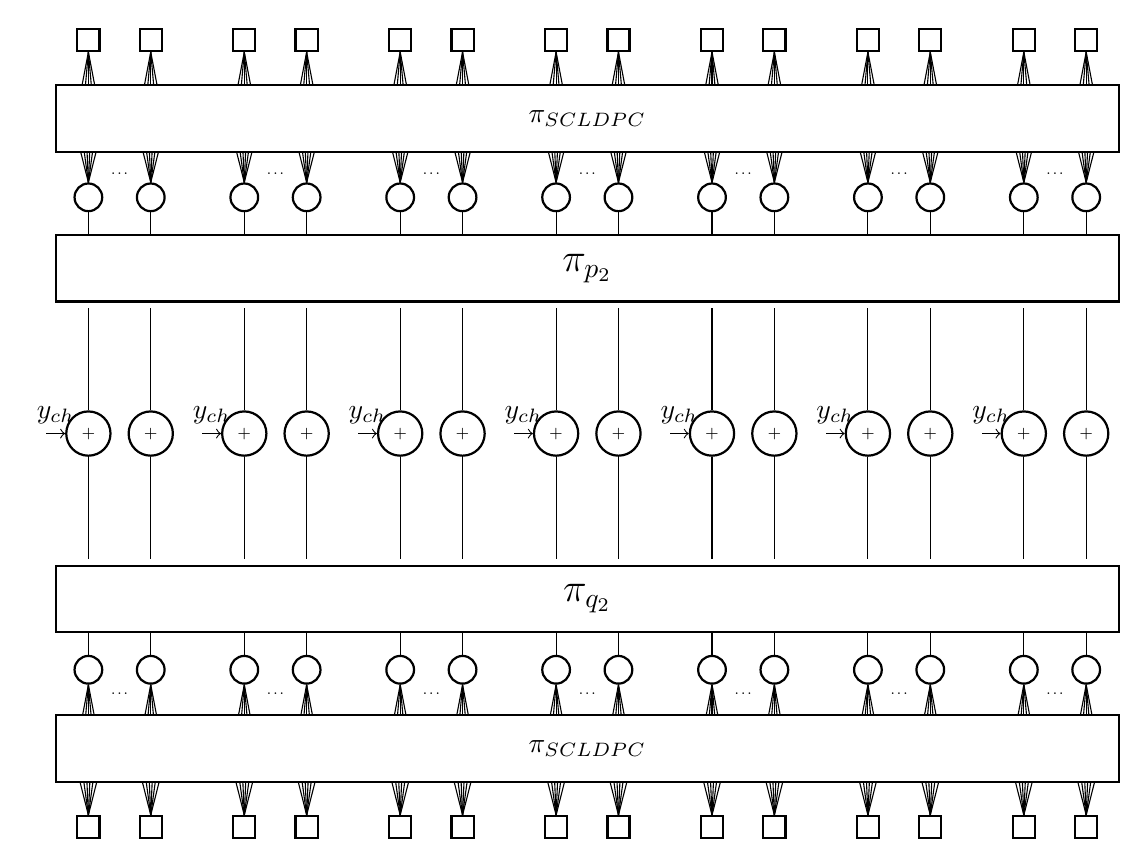
\begin{tikzpicture}[
  xscale=0.33,yscale=1,
  bitnode/.style={circle,minimum size=10pt,thick,draw=black,fill=white},
  bitnodeblack/.style={circle,minimum size=10pt,thick,draw=black,fill=white},
  bitnodewhite/.style={circle,minimum size=10pt,thick,draw=white,fill=gray},
  bitnode2/.style={circle,minimum size=10pt,thick,draw=black,fill=gray},
  bitnode2black/.style={circle,minimum size=10pt,thick,draw=black,fill=gray},
  bitnode2white/.style={circle,minimum size=10pt,thick,draw=white,fill=white},
  checknode/.style={rectangle,minimum size=8pt,thick,draw=black,fill=white},
  checknodeblack/.style={rectangle,minimum size=8pt,thick,draw=black,fill=white},
  checknodewhite/.style={rectangle,minimum size=8pt,thick,draw=white,fill=white},
  permnode/.style={rectangle,very thin,minimum width=30pt,minimum height=18pt,fill=white,draw=black},
  permnodeblack/.style={rectangle,very thin,minimum width=30pt,minimum height=18pt,fill=white,draw=black},
  permnodewhite/.style={rectangle,very thin,minimum width=30pt,minimum height=18pt,fill=white,draw=white},
  permedge/.style={black!65},
  permedgeblack/.style={black!65},
  permedgewhite/.style={white},
  ]

  \def \cndist {1.2}
  \def \vndist {1.2}
  \def \ccndist {1.2}
  \def \vvny {2.75}
  \def \cny {3}
  \def \vny {1}
  \def \vnya {-2}
  \def \vnyb {-5}
  \def \ccny {-7}
    \def \ext{1.3}
      \def \exta {1}
  \def \midx   {0.5}
  
    \tikzstyle{bigPerm}= [rectangle, draw, thick, minimum width=320*\vndist, minimum height=20*\vndist,fill=white, draw=black]
    
\def\ldgcol{black}
\def\ldpcol{black}
\def\seqa{black}
\def\seqb{black}
    \foreach \x/\i in {0/1,6/2,12/3,18/4,24/5,30/6,36/7} {

      \node[bitnode\seqa] (v1\i) at (\x-\vndist, \vny) {};
      \node[bitnode\seqa] (v2\i) at (\x+\vndist, \vny) {};
      \node at (\x,\vny+0.3) {\tiny{$...$}};
% Edges- LDPC bits to top
      \draw[\seqa] (v1\i.north) -- +(52.5:1);
      \draw[\seqa] (v1\i.north) -- +(67.5:1);
      \draw[\seqa] (v1\i.north) -- +(82.5:1);
      \draw[\seqa] (v1\i.north) -- +(97.5:1);
      \draw[\seqa] (v1\i.north) -- +(112.5:1);
      \draw[\seqa] (v1\i.north) -- +(127.5:1);

      \draw[\seqa] (v2\i.north) -- +(52.5:1);
      \draw[\seqa] (v2\i.north) -- +(67.5:1);
      \draw[\seqa] (v2\i.north) -- +(82.5:1);
      \draw[\seqa] (v2\i.north) -- +(97.5:1);
      \draw[\seqa] (v2\i.north) -- +(112.5:1);
      \draw[\seqa] (v2\i.north) -- +(127.5:1);


     \node[bitnode\seqb] (v3\i) at (\x-\vndist, \vnyb) {};
     \node[bitnode\seqb] (v4\i) at (\x+\vndist, \vnyb) {};
     \node at (\x,\vnyb-0.3) {\tiny{$...$}};
     
% Edges- LDPC bits to bottom
      \draw[\seqb] (v3\i.south) -- +(240:1);
      \draw[\seqb] (v3\i.south) -- +(255:1);
      \draw[\seqb] (v3\i.south) -- +(270:1);
      \draw[\seqb] (v3\i.south) -- +(285:1);
      \draw[\seqb] (v3\i.south) -- +(300:1);

      \draw[\seqb] (v4\i.south) -- +(240:1);
      \draw[\seqb] (v4\i.south) -- +(255:1);
      \draw[\seqb] (v4\i.south) -- +(270:1);
      \draw[\seqb] (v4\i.south) -- +(285:1);
      \draw[\seqb] (v4\i.south) -- +(300:1);

% Middle bits= Actual GMAC Code bits
    \node[bitnode] (v5\i) at (\x-\vndist, \vnya) {\tiny $+$};
    \node[bitnode] (v6\i) at (\x+\vndist, \vnya) {\tiny $+$};
     

    \draw (v1\i.south) -- +(270:\exta);      \draw (v2\i.south) -- +(270:\exta);    
    \draw (v3\i.north) -- +(90:\exta);        \draw (v4\i.north) -- +(90:\exta);

    \draw (v5\i.north)-- +(90:\ext);       \draw (v6\i.north)-- +(90:\ext);
    \draw (v5\i.south) -- +(270:\ext);    \draw (v6\i.south) -- +(270:\ext);

    \draw[<-] (v5\i.west) -- node[midway, above]{$y_{\text{ch}}$} +(-0.6*\vndist,0);

% Top Checks
 \node[checknode\ldgcol] (c1\i) at (\x-\cndist, \cny) {};
  \node[checknode\ldgcol] (c2\i) at (\x+\cndist, \cny) {};

% Top check to bottom
      \draw[\ldgcol] (c1\i.south) -- +(240:1);
      \draw[\ldgcol] (c1\i.south) -- +(255:1);
      \draw[\ldgcol] (c1\i.south) -- +(270:1);
      \draw[\ldgcol] (c1\i.south) -- +(285:1);
      \draw[\ldgcol] (c1\i.south) -- +(300:1);

      \draw[\ldgcol] (c2\i.south) -- +(240:1);
      \draw[\ldgcol] (c2\i.south) -- +(255:1);
      \draw[\ldgcol] (c2\i.south) -- +(270:1);
      \draw[\ldgcol] (c2\i.south) -- +(285:1);
      \draw[\ldgcol] (c2\i.south) -- +(300:1);

  
%Bottom Checks  
      \node[checknode\ldpcol] (cc1\i) at (\x-\ccndist, \ccny) {};
      \node[checknode\ldpcol] (cc2\i) at (\x+\ccndist, \ccny) {};
      
% Bottom checks to top
      \draw[\ldpcol] (cc1\i.north) -- +(52.5:1);
      \draw[\ldpcol] (cc1\i.north) -- +(67.5:1);
      \draw[\ldpcol] (cc1\i.north) -- +(82.5:1);
      \draw[\ldpcol] (cc1\i.north) -- +(97.5:1);
      \draw[\ldpcol] (cc1\i.north) -- +(112.5:1);
      \draw[\ldpcol] (cc1\i.north) -- +(127.5:1);

      \draw[\ldpcol] (cc2\i.north) -- +(52.5:1);
      \draw[\ldpcol] (cc2\i.north) -- +(67.5:1);
      \draw[\ldpcol] (cc2\i.north) -- +(82.5:1);
      \draw[\ldpcol] (cc2\i.north) -- +(97.5:1);
      \draw[\ldpcol] (cc2\i.north) -- +(112.5:1);
      \draw[\ldpcol] (cc2\i.north) -- +(127.5:1);

      \node[\ldpcol] at (\x,-5.7) {\tiny{$...$}};
      \node[\ldgcol] at (\x,1.7) {\tiny{$...$}};

}

  \node[bigPerm] (perm1_node) at (18,0.5*\vny+0.5*\cny) {\normalsize $\pi_{\text{SCLDPC}}$};    
  \node[bigPerm] (perm2_node) at (18,0.5*\vnyb+0.5*\ccny) {\normalsize $\pi_{\text{SCLDPC}}$};    
  
  \node[bigPerm] (perm3_node) at (18,0.7*\vny+0.3*\vnya) {\Large $\pi_{p_2}$};    
  \node[bigPerm] (perm4_node) at (18,0.3*\vnya+0.7*\vnyb) {\Large $\pi_{q_2}$};    
   
\end{tikzpicture}}
}
\end{frame}

%%%%%%%%%%%%----------------------------------------------------------------------------------%%%%%%%%%%%%%%%
\begin{frame}\frametitle{Decoding in a slot: Belief propagation for MAC }
\begin{itemize}
\item Message passing rules at bit/check nodes identical to single user
\onslide<2->{
\item Message passing rule at GMAC node:
\begin{align*}
v^{1}_{\text{MAC},i}&=h(u^{2}_{i,\text{MAC}},y_{i,\text{ch}})\\
v^{2}_{i,\text{MAC}}&=h(u^{1}_{i,\text{MAC}},y_{i,\text{ch}}) ~~~\text{ where}\notag\\
h(l,y)&=\log \frac{1+e^{l}e^{2(y-1)/\sigma^2}}{e^{l}+e^{-2(y+1)/\sigma^2}}
\end{align*}
}
\end{itemize}

	\centering
	\vspace{2ex}
	\resizebox{0.85\textwidth}{!}{\begin{tikzpicture}
\def \depth{1.5}; %vertical gap between nodes/levels
\def \xgap{2.8}
\def \gap{0.6}; %Horizontal gap between nodes
\def \gapA{0.3}; %Encoder Width
\def \textoffs{0.24}; %Offset for writing text above a node
\def\nodewidth{0.5};
\tikzstyle{bitwhite} = [circle, draw, thick, fill=white, radius=0.5*\nodewidth]
\tikzstyle{bitshaded} = [circle, draw, thick, fill=gray, radius=0.5*\nodewidth]
\tikzstyle{checkwhite} = [rectangle, draw, thick, fill=white,minimum height=\nodewidth, minimum width=\nodewidth]
\tikzstyle{checkshaded} = [rectangle, draw, thick, fill=gray,minimum height=\nodewidth, minimum width=\nodewidth]
                          
\def \fsize{\footnotesize}; %Defining a generic font size to be adjusted depending on the scaling
\def \fsizea{\tiny}; %Defining a generic font size to be adjusted depending on the scaling
\def \dotsize{\Huge}; %Defining a generic font size to be adjusted depending on the scaling

%%---------------------- Graph 1---------------------------------------------------------------------------
\node [bitshaded](b1) at (0,0) {\fsizea $i$} ;
\node [bitwhite,radius=0.8*\nodewidth](bMAC) at (0,1) {\fsize $+$} ;
\draw[thick,decoration={markings,mark=at position 0.5 with {\arrow{>}}},postaction={decorate}] (b1.north) -- node[midway,left]{{\fsize $u_{i,\text{MAC}}$}} node[midway,right] {\fsize $=\sum\limits_{j=1}^{3}v_{j,i}$} (bMAC.south);

\foreach \i in {1,2,3}
{
\path (b1) -- +(180+\i*45:\depth) node[checkwhite] (c1\i) {\fsize $\i$};
\begin{scope}[decoration={ markings,    mark=at position 0.5 with {\arrow{>}}} ] 
\draw[postaction=decorate] (c1\i.north) -- node[pos=0.3,left]{{\fsize $v_{\i,i}$}} (b1);
\end{scope}
}

%%---------------------- Graph 2---------------------------------------------------------------------------
\node [bitshaded,radius=0.5*\nodewidth](bMAC2) at (\xgap,0) {\fsize $+$} ;
\node [bitwhite](b2) at (\xgap,1) {\fsizea $i$} ;
%\node () at (b2.east) {\fsizea User 2} ;
\draw[decoration={markings,mark=at position 0.5 with {\arrow{>}}},postaction={decorate}] (b2.south) -- node[midway,left]{{\fsize $u^{2}_{i,\text{MAC}}$}} (bMAC2.north);
\draw[decoration={markings,mark=at position 0.5 with {\arrow{<}}},postaction={decorate}] (bMAC2.west) -- node[midway,below]{{\fsize $y_{i,\text{ch}}$}} +(-0.25*\xgap,0);


\path (bMAC2) -- +(180+90:\depth) node[bitwhite] (b21) {\fsizea $i$};
\draw[thick,decoration={ markings, mark=at position 0.5 with {\arrow{<}}}, postaction=decorate] (b21.north) -- node[midway,left]{{\fsize $v^{1}_{\text{MAC},i}$}} (bMAC2);


%%---------------------- Graph 3---------------------------------------------------------------------------
\node [bitshaded](b3) at (2*\xgap,0) {\fsizea $i$} ;
\node [bitwhite,radius=0.8*\nodewidth](bMAC3) at (2*\xgap,1) {\fsize $+$} ;
\draw[decoration={markings,mark=at position 0.5 with {\arrow{<}}},postaction={decorate}] (b3.north) -- node[midway,left]{{\fsize $v_{\text{MAC},i}$}} (bMAC3.south);

\foreach \i in {1,2,3}
{
\path (b3) -- +(180+\i*45:\depth) node[checkwhite] (c3\i) {\fsize $\i$};
}
\foreach \i in {1,2}
{
\draw[decoration={ markings, mark=at position 0.5 with {\arrow{>}}}, postaction=decorate] (c3\i.north) -- node[pos=0.3,left]{{\fsize $v_{\i,i}$}} (b3.south);
}
\draw[thick,decoration={ markings, mark=at position 0.6 with {\arrow{<}}}, postaction=decorate] (c33.north) -- node[midway,right]{{\fsize $u_{i,3}=v_{\text{MAC},i}+\sum\limits_{j=1}^{2}v_{j,i}$}} (b3.south);

\end{tikzpicture}}
\end{frame}

%%%%%%%%%%%%----------------------------------------------------------------------------------%%%%%%%%%%%%%%%
%\begin{frame}\frametitle{Decoder across slots: Peeling}
%\begin{itemize}
%\item Given $\yv_j=\xv_{w_i}+\zv_j$, assume we can decode $\xv_{w_i}$
%\end{itemize}
%\centering
%\resizebox{0.4\textwidth}{!}{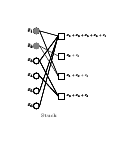
\begin{tikzpicture}
\def\horzgap{0.125in}; %Horizontal gap between nodes/levels
\def \gapVN{0.075in}; %vertical gap between nodes
\def \gapCN{0.1in}; %Horizontal gap between nodes


\def\nodewidth{0.5ex}; 
\def\nodewidthA{0.5ex};
\def \edgewidth{15ex}; 
\def\ext{0.1in};


\tikzstyle{check} = [rectangle, draw,line width=0.07mm, inner sep=0mm, minimum height=\nodewidthA, minimum width=\nodewidthA]
\tikzstyle{bit} = [circle, draw, line width=0.07mm, inner sep=0mm,  minimum size=\nodewidthA]
\tikzstyle{bituncover} = [circle, draw=none, line width=0.05mm, inner sep=0mm, fill=gray, minimum size=\nodewidthA]

 \def\moveX {1.8*\nodewidth};
\def\moveXA {2*\nodewidth};

            
\onslide<1>{             
\foreach \vn in {1,...,6}{
 \node[bit] (vn\vn) at (0,-\vn*\gapVN) {};
}

\foreach \vn in {1,...,6}{
\path (vn\vn) ++(-\nodewidth,0) node()[scale=0.25, inner sep=0mm] {\tiny{$\vec{x}_{\vn}$}};
}

\foreach \cn in {1,...,4}{
\node[check] (cn\cn) at (\horzgap,-\cn*\gapCN) {};
}

\draw[line width=0.05mm] (vn4.east)--(cn4.west);
\draw[line width=0.05mm] (vn3.east)--(cn4.west);

\draw[line width=0.05mm] (vn2.east)--(cn3.west);
\draw[line width=0.05mm] (vn1.east)--(cn3.west);

\draw[line width=0.05mm] (vn2.east)--(cn2.west);

\draw[line width=0.05mm] (vn1.east)--(cn1.west);
\draw[line width=0.05mm] (vn3.east)--(cn1.west);
\draw[line width=0.05mm] (vn5.east)--(cn1.west);
\draw[line width=0.05mm] (vn6.east)--(cn1.west);


\node [scale=0.2,anchor=west] at (cn1.east) {\tiny{$\vec{x}_1+\vec{x}_3+\vec{x}_5+\vec{x}_6+\vec{z}_1$}};
\node [scale=0.2,anchor=west] at (cn2.east) {\tiny{$\vec{x}_2+\vec{z}_2$}};
\node [scale=0.2,anchor=west] at (cn3.east) {\tiny{$\vec{x}_1+\vec{x}_2+\vec{z}_3$}};
\node [scale=0.2,anchor=west] at (cn4.east) {\tiny{$\vec{x}_3+\vec{x}_4+\vec{z}_4$}};

}

%-----------------------*(&^#@$^&*(^%$^&*(&^--------------------------------------------------------------------
%Dotted x_2
\onslide<2>{
\foreach \vn in {1,3,4,5,6}{
 \node[bit] (vn\vn) at (0,-\vn*\gapVN) {};
}

\foreach \vn in {1,3,4,5,6}{
\path (vn\vn) ++(-\nodewidth,0) node()[scale=0.25, inner sep=0mm] {\tiny{$\vec{x}_{\vn}$}};
}


\foreach \vn in {2}{
 \node[bituncover] (vn\vn) at (0,-\vn*\gapVN) {};
}

\foreach \vn in {2}{
\path (vn\vn) ++(-\nodewidth,0) node()[scale=0.25, inner sep=0mm] {\tiny{$\hat{\vec{x}}_2$}};
}


\foreach \cn in {1,...,4}{
\node[check] (cn\cn) at (\horzgap,-\cn*\gapCN) {};
}


\draw[line width=0.05mm] (vn4.east)--(cn4.west);
\draw[line width=0.05mm] (vn3.east)--(cn4.west);

\draw[line width=0.05mm, densely dotted] (vn2.east)--(cn3.west);
\draw[line width=0.05mm] (vn1.east)--(cn3.west);

\draw[line width=0.05mm, densely dotted] (vn2.east)--(cn2.west);

\draw[line width=0.05mm] (vn1.east)--(cn1.west);
\draw[line width=0.05mm] (vn3.east)--(cn1.west);
\draw[line width=0.05mm] (vn5.east)--(cn1.west);
\draw[line width=0.05mm] (vn6.east)--(cn1.west);

\node [scale=0.2,anchor=west] at (cn1.east) {\tiny{$\vec{x}_1+\vec{x}_3+\vec{x}_5+\vec{x}_6+\vec{z}_1$}};
\node [scale=0.2,anchor=west] at (cn2.east) {\tiny{$\vec{x}_2+\vec{z}_2$}};
\node [scale=0.2,anchor=west] at (cn3.east) {\tiny{$\vec{x}_1+\vec{x}_2+\vec{z}_3$}};
\node [scale=0.2,anchor=west] at (cn4.east) {\tiny{$\vec{x}_3+\vec{x}_4+\vec{z}_4$}};
}
%----------------------------------^%$#@%^&*()_*&^%$#^&*------------------------------------
%--Peeled x_2
\onslide<3>{
\foreach \vn in {1,3,4,5,6}{
 \node[bit] (vn\vn) at (0,-\vn*\gapVN) {};
}

\foreach \vn in {1,3,4,5,6}{
\path (vn\vn) ++(-\nodewidth,0) node()[scale=0.25, inner sep=0mm] {\tiny{$\vec{x}_{\vn}$}};
}


\foreach \vn in {2}{
 \node[bituncover] (vn\vn) at (0,-\vn*\gapVN) {};
}

\foreach \vn in {2}{
\path (vn\vn) ++(-\nodewidth,0) node()[scale=0.25, inner sep=0mm] {\tiny{$\hat{\vec{x}}_2$}};
}


\foreach \cn in {1,...,4}{
\node[check] (cn\cn) at (\horzgap,-\cn*\gapCN) {};
}


\draw[line width=0.05mm] (vn4.east)--(cn4.west);
\draw[line width=0.05mm] (vn3.east)--(cn4.west);

\draw[line width=0.05mm] (vn1.east)--(cn3.west);

\draw[line width=0.05mm] (vn1.east)--(cn1.west);
\draw[line width=0.05mm] (vn3.east)--(cn1.west);
\draw[line width=0.05mm] (vn5.east)--(cn1.west);
\draw[line width=0.05mm] (vn6.east)--(cn1.west);

\node [scale=0.2,anchor=west] at (cn1.east) {\tiny{$\vec{x}_1+\vec{x}_3+\vec{x}_5+\vec{x}_6+\vec{z}_1$}};
\node [scale=0.2,anchor=west] at (cn2.east) {\tiny{$\vec{z}_2$}};
\node [scale=0.2,anchor=west] at (cn3.east) {\tiny{$\vec{x}_1+\vec{z}_3$}};
\node [scale=0.2,anchor=west] at (cn4.east) {\tiny{$\vec{x}_3+\vec{x}_4+\vec{z}_4$}};
}

%---------%^&*^%$#^&----------------------------
%Dotted x_1
\onslide<4>{
\foreach \vn in {3,4,5,6}{
 \node[bit] (vn\vn) at (0,-\vn*\gapVN) {};
}

\foreach \vn in {1,2}{
 \node[bituncover] (vn\vn) at (0,-\vn*\gapVN) {};
}


\foreach \vn in {3,4,5,6}{
\path (vn\vn) ++(-\nodewidth,0) node()[scale=0.25, inner sep=0mm] {\tiny{$\vec{x}_{\vn}$}};
}

\foreach \vn in {1,2}{
\path (vn\vn) ++(-\nodewidth,0) node()[scale=0.25, inner sep=0mm] {\tiny{$\hat{\vec{x}}_{\vn}$}};
}

\foreach \cn in {1,...,4}{
\node[check] (cn\cn) at (\horzgap,-\cn*\gapCN) {};
}


\draw[line width=0.05mm] (vn4.east)--(cn4.west);
\draw[line width=0.05mm] (vn3.east)--(cn4.west);

\draw[line width=0.05mm, densely dotted] (vn1.east)--(cn3.west);
\draw[line width=0.05mm, densely dotted] (vn1.east)--(cn1.west);

\draw[line width=0.05mm] (vn3.east)--(cn1.west);
\draw[line width=0.05mm] (vn5.east)--(cn1.west);
\draw[line width=0.05mm] (vn6.east)--(cn1.west);


\node [scale=0.2,anchor=west] at (cn1.east) {\tiny{$\vec{x}_1+\vec{x}_3+\vec{x}_5+\vec{x}_6+\vec{z}_1$}};
\node [scale=0.2,anchor=west] at (cn2.east) {\tiny{$\vec{z}_2$}};
\node [scale=0.2,anchor=west] at (cn3.east) {\tiny{$\vec{x}_1+\vec{z}_3$}};
\node [scale=0.2,anchor=west] at (cn4.east) {\tiny{$\vec{x}_3+\vec{x}_4+\vec{z}_4$}};
}

%----------------------------------^%$#@%^&*()_*&^%$#^&*------------------------------------
%-peeled off x_1
\onslide<5>{
\foreach \vn in {3,4,5,6}{
 \node[bit] (vn\vn) at (0,-\vn*\gapVN) {};
}

\foreach \vn in {1,2}{
 \node[bituncover] (vn\vn) at (0,-\vn*\gapVN) {};
}


\foreach \vn in {3,4,5,6}{
\path (vn\vn) ++(-\nodewidth,0) node()[scale=0.25, inner sep=0mm] {\tiny{$\vec{x}_{\vn}$}};
}

\foreach \vn in {1,2}{
\path (vn\vn) ++(-\nodewidth,0) node()[scale=0.25, inner sep=0mm] {\tiny{$\hat{\vec{x}}_{\vn}$}};
}

\foreach \cn in {1,...,4}{
\node[check] (cn\cn) at (\horzgap,-\cn*\gapCN) {};
}


\draw[line width=0.05mm] (vn4.east)--(cn4.west);
\draw[line width=0.05mm] (vn3.east)--(cn4.west);

\draw[line width=0.05mm] (vn3.east)--(cn1.west);
\draw[line width=0.05mm] (vn5.east)--(cn1.west);
\draw[line width=0.05mm] (vn6.east)--(cn1.west);


\node [scale=0.2,anchor=west] at (cn1.east) {\tiny{$\vec{x}_3+\vec{x}_5+\vec{x}_6+\vec{z}_1$}};
\node [scale=0.2,anchor=west] at (cn2.east) {\tiny{$\vec{z}_2$}};
\node [scale=0.2,anchor=west] at (cn3.east) {\tiny{$\vec{z}_3$}};
\node [scale=0.2,anchor=west] at (cn4.east) {\tiny{$\vec{x}_3+\vec{x}_4+\vec{z}_4$}};
}

%----------------------------------^%$#@%^&*()_*&^%$#^&*------------------------------------
\onslide<6>{
\foreach \vn in {3,4,5,6}{
 \node[bit] (vn\vn) at (0,-\vn*\gapVN) {};
}

\foreach \vn in {1,2}{
 \node[bituncover] (vn\vn) at (0,-\vn*\gapVN) {};
}


\foreach \vn in {3,4,5,6}{
\path (vn\vn) ++(-\nodewidth,0) node()[scale=0.25, inner sep=0mm] {\tiny{$\vec{x}_{\vn}$}};
}

\foreach \vn in {1,2}{
\path (vn\vn) ++(-\nodewidth,0) node()[scale=0.25, inner sep=0mm] {\tiny{$\hat{\vec{x}}_{\vn}$}};
}

\foreach \cn in {1,...,4}{
\node[check] (cn\cn) at (\horzgap,-\cn*\gapCN) {};
}


\draw[line width=0.05mm] (vn4.east)--(cn4.west);
\draw[line width=0.05mm] (vn3.east)--(cn4.west);

\draw[line width=0.05mm] (vn3.east)--(cn1.west);
\draw[line width=0.05mm] (vn5.east)--(cn1.west);
\draw[line width=0.05mm] (vn6.east)--(cn1.west);


\node [scale=0.2,anchor=west] at (cn1.east) {\tiny{$\vec{x}_3+\vec{x}_5+\vec{x}_6+\vec{z}_1$}};
\node [scale=0.2,anchor=west] at (cn2.east) {\tiny{$\vec{z}_2$}};
\node [scale=0.2,anchor=west] at (cn3.east) {\tiny{$\vec{z}_3$}};
\node [scale=0.2,anchor=west] at (cn4.east) {\tiny{$\vec{x}_3+\vec{x}_4+\vec{z}_4$}};

\node[scale=0.35] () at (0.5*\horzgap,-5*\gapCN) {\tiny{Stuck}};
}
\end{tikzpicture}}
%\end{frame}

%%%%%%%%%%%%----------------------------------------------------------------------------------%%%%%%%%%%%%%%%
\begin{frame}
\frametitle{Decoder across slots: $T$-Peeling}
%\begin{itemize}
%\item In slot $j$, assume we can decode $\{\xv_{w_i},i\in\mc{N}_j\}$ if $|\mc{N}_j|\leq T$
%\[
%\yv_j=\sum\limits_{i\in\mc{N}_j}\xv_{w_i}+\zv_j
%\]
%\end{itemize}
\centering
\resizebox{0.85\textwidth}{!}{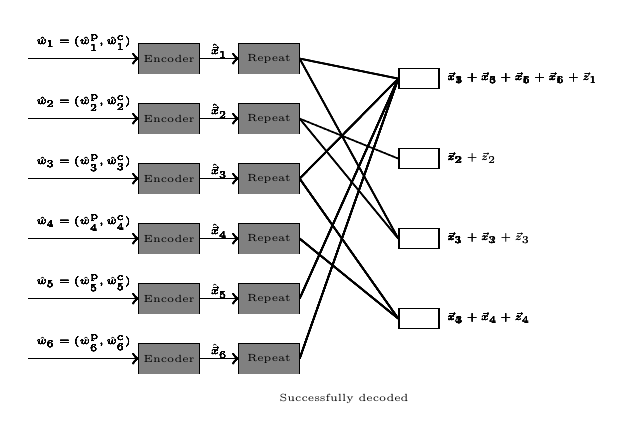
\begin{tikzpicture}
\def\horzgap{0.75in}; %Horizontal gap between nodes/levels
\def \gapVN{0.3in}; %vertical gap between nodes
\def \gapCN{0.4in}; %Horizontal gap between nodes
\def\fsize{\tiny}
\def\fac{0.75}
\def\lw{0.2mm}

\def\nodewidth{0.1in}; 
\def\nodewidthA{0.2in};
\def \edgewidth{15ex}; 
\def\ext{0.5in};


\tikzstyle{check} = [rectangle, draw,line width=\lw, inner sep=0mm, minimum height=\nodewidth, minimum width=2*\nodewidth]
\tikzstyle{block} = [rectangle, draw, line width=\lw, inner sep=0mm,  minimum height=\nodewidthA, minimum width=2*\nodewidthA]
\tikzstyle{bit} = [circle, draw, line width=\lw, inner sep=0mm,  minimum size=\nodewidthA]
\tikzstyle{blockuncover} = [rectangle, draw=none, fill=gray, line width=\lw, inner sep=0mm,  minimum height=\nodewidthA, minimum width=2*\nodewidthA]

 \def\moveX {1.8*\nodewidth};
\def\moveXA {2*\nodewidth};



\onslide<1>{             

\foreach \vn in {1,...,6}{
\node[block,scale=\fac] (vn\vn) at (0,-\vn*\gapVN) {\tiny{Repeat}};
\path (vn\vn)++(-\ext,0) node[scale=\fac,block] (vna\vn) {\tiny{Encoder}};
\draw[->,line width=\lw] (vna\vn.east)--node[midway,above,scale=\fac, inner sep=0mm] {\fsize{$\vec{x}_{\vn}$}} (vn\vn.west);
\draw[<-, line width=\lw] (vna\vn.west)--node[midway, above,scale=\fac]{\fsize{$w_{\vn} =(w_{\vn}^{\mathrm{p}}, w_{\vn}^{\mathrm{c}})$}}+(-1.1*\ext,0);
}

\foreach \cn in {1,...,4}{
\node[check] (cn\cn) at (\horzgap,-\cn*\gapCN) {};
}

\draw[line width=\lw] (vn4.east)--(cn4.west);
\draw[line width=\lw] (vn3.east)--(cn4.west);

\draw[line width=\lw] (vn2.east)--(cn3.west);
\draw[line width=\lw] (vn1.east)--(cn3.west);

\draw[line width=\lw] (vn2.east)--(cn2.west);

\draw[line width=\lw] (vn1.east)--(cn1.west);
\draw[line width=\lw] (vn3.east)--(cn1.west);
\draw[line width=\lw] (vn5.east)--(cn1.west);
\draw[line width=\lw] (vn6.east)--(cn1.west);


\node [scale=\fac,anchor=west] at (cn1.east) {\fsize{$\vec{x}_1+\vec{x}_3+\vec{x}_5+\vec{x}_6+\vec{z}_1$}};
\node [scale=\fac,anchor=west] at (cn2.east) {\fsize{$\vec{x}_2+\vec{z}_2$}};
\node [scale=\fac,anchor=west] at (cn3.east) {\fsize{$\vec{x}_1+\vec{x}_2+\vec{z}_3$}};
\node [scale=\fac,anchor=west] at (cn4.east) {\fsize{$\vec{x}_3+\vec{x}_4+\vec{z}_4$}};
}

%%-----------------------*(&^#@$^&*(^%$^&*(&^--------------------------------------------------------------------
%Dotted x_2

\onslide<2>{

\foreach \vn in {1,3,4,5,6}{
\node[block,scale=\fac] (vn\vn) at (0,-\vn*\gapVN) {\tiny{Repeat}};
\path (vn\vn)++(-\ext,0) node[scale=\fac,block] (vna\vn) {\tiny{Encoder}};
\draw[->,line width=\lw] (vna\vn.east)--node[midway,above,scale=\fac, inner sep=0mm] {\fsize{$\vec{x}_{\vn}$}} (vn\vn.west);
\draw[<-, line width=\lw] (vna\vn.west)--node[midway, above,scale=\fac]{\fsize{$w_{\vn} =(w_{\vn}^{\mathrm{p}}, w_{\vn}^{\mathrm{c}})$}}+(-1.1*\ext,0);
}


\foreach \vn in {2}{
\node[blockuncover,scale=\fac] (vn\vn) at (0,-\vn*\gapVN) {\tiny{Repeat}};
\path (vn\vn)++(-\ext,0) node[scale=\fac,blockuncover] (vna\vn) {\tiny{Encoder}};
\draw[->,line width=\lw] (vna\vn.east)--node[midway,above,scale=\fac, inner sep=0mm] {\fsize{$\hat{\vec{x}}_{\vn}$}} (vn\vn.west);
\draw[<-, line width=\lw] (vna\vn.west)--node[midway, above,scale=\fac]{\fsize{$\hat{w}_{\vn} =(\hat{w}_{\vn}^{\mathrm{p}},\hat{w}_{\vn}^{\mathrm{c}})$}}+(-1.1*\ext,0);
}

\foreach \cn in {1,...,4}{
\node[check] (cn\cn) at (\horzgap,-\cn*\gapCN) {};
}


\draw[line width=\lw] (vn4.east)--(cn4.west);
\draw[line width=\lw] (vn3.east)--(cn4.west);

\draw[line width=\lw] (vn2.east)--(cn3.west);
\draw[line width=\lw] (vn1.east)--(cn3.west);

\draw[line width=\lw, densely dotted] (vn2.east)--(cn2.west);

\draw[line width=\lw] (vn1.east)--(cn1.west);
\draw[line width=\lw] (vn3.east)--(cn1.west);
\draw[line width=\lw] (vn5.east)--(cn1.west);
\draw[line width=\lw] (vn6.east)--(cn1.west);

\node [scale=\fac,anchor=west] at (cn1.east) {\tiny{$\vec{x}_1+\vec{x}_3+\vec{x}_5+\vec{x}_6+\vec{z}_1$}};
\node [scale=\fac,anchor=west] at (cn2.east) {\tiny{$\vec{x}_2+\vec{z}_2$}};
\node [scale=\fac,anchor=west] at (cn3.east) {\tiny{$\vec{x}_1+\vec{x}_2+\vec{z}_3$}};
\node [scale=\fac,anchor=west] at (cn4.east) {\tiny{$\vec{x}_3+\vec{x}_4+\vec{z}_4$}};
}

%%----------------------------------^%$#@%^&*()_*&^%$#^&*------------------------------------
%%--Peeled x_2
\onslide<3>{

\foreach \vn in {1,3,4,5,6}{
\node[block,scale=\fac] (vn\vn) at (0,-\vn*\gapVN) {\tiny{Repeat}};
\path (vn\vn)++(-\ext,0) node[scale=\fac,block] (vna\vn) {\tiny{Encoder}};
\draw[->,line width=\lw] (vna\vn.east)--node[midway,above,scale=\fac, inner sep=0mm] {\fsize{$\vec{x}_{\vn}$}} (vn\vn.west);
\draw[<-, line width=\lw] (vna\vn.west)--node[midway, above,scale=\fac]{\fsize{$w_{\vn} =(w_{\vn}^{\mathrm{p}}, w_{\vn}^{\mathrm{c}})$}}+(-1.1*\ext,0);
}


\foreach \vn in {2}{
\node[blockuncover,scale=\fac] (vn\vn) at (0,-\vn*\gapVN) {\tiny{Repeat}};
\path (vn\vn)++(-\ext,0) node[scale=\fac,blockuncover] (vna\vn) {\tiny{Encoder}};
\draw[->,line width=\lw] (vna\vn.east)--node[midway,above,scale=\fac, inner sep=0mm] {\fsize{$\hat{\vec{x}}_{\vn}$}} (vn\vn.west);
\draw[<-, line width=\lw] (vna\vn.west)--node[midway, above,scale=\fac]{\fsize{$\hat{w}_{\vn} =(\hat{w}_{\vn}^{\mathrm{p}},\hat{w}_{\vn}^{\mathrm{c}})$}}+(-1.1*\ext,0);
}


\foreach \cn in {1,...,4}{
\node[check] (cn\cn) at (\horzgap,-\cn*\gapCN) {};
}


\draw[line width=\lw] (vn4.east)--(cn4.west);
\draw[line width=\lw] (vn3.east)--(cn4.west);

\draw[line width=\lw] (vn1.east)--(cn3.west);

\draw[line width=\lw] (vn1.east)--(cn1.west);
\draw[line width=\lw] (vn3.east)--(cn1.west);
\draw[line width=\lw] (vn5.east)--(cn1.west);
\draw[line width=\lw] (vn6.east)--(cn1.west);

\node [scale=\fac,anchor=west] at (cn1.east) {\tiny{$\vec{x}_1+\vec{x}_3+\vec{x}_5+\vec{x}_6+\vec{z}_1$}};
\node [scale=\fac,anchor=west] at (cn2.east) {\tiny{$\vec{z}_2$}};
\node [scale=\fac,anchor=west] at (cn3.east) {\tiny{$\vec{x}_1+\vec{z}_3$}};
\node [scale=\fac,anchor=west] at (cn4.east) {\tiny{$\vec{x}_3+\vec{x}_4+\vec{z}_4$}};
}

%%---------%^&*^%$#^&----------------------------
%%Dotted x_1
\onslide<4>{

\foreach \vn in {3,4,5,6}{
\node[block,scale=\fac] (vn\vn) at (0,-\vn*\gapVN) {\tiny{Repeat}};
\path (vn\vn)++(-\ext,0) node[scale=\fac,block] (vna\vn) {\tiny{Encoder}};
\draw[->,line width=\lw] (vna\vn.east)--node[midway,above,scale=\fac, inner sep=0mm] {\fsize{$\vec{x}_{\vn}$}} (vn\vn.west);
\draw[<-, line width=\lw] (vna\vn.west)--node[midway, above,scale=\fac]{\fsize{$w_{\vn} =(w_{\vn}^{\mathrm{p}}, w_{\vn}^{\mathrm{c}})$}}+(-1.1*\ext,0);
}


\foreach \vn in {1,2}{
\node[blockuncover,scale=\fac] (vn\vn) at (0,-\vn*\gapVN) {\tiny{Repeat}};
\path (vn\vn)++(-\ext,0) node[scale=\fac,blockuncover] (vna\vn) {\tiny{Encoder}};
\draw[->,line width=\lw] (vna\vn.east)--node[midway,above,scale=\fac, inner sep=0mm] {\fsize{$\hat{\vec{x}}_{\vn}$}} (vn\vn.west);
\draw[<-, line width=\lw] (vna\vn.west)--node[midway, above,scale=\fac]{\fsize{$\hat{w}_{\vn} =(\hat{w}_{\vn}^{\mathrm{p}},\hat{w}_{\vn}^{\mathrm{c}})$}}+(-1.1*\ext,0);
}


\foreach \cn in {1,...,4}{
\node[check] (cn\cn) at (\horzgap,-\cn*\gapCN) {};
}


\draw[line width=\lw] (vn4.east)--(cn4.west);
\draw[line width=\lw] (vn3.east)--(cn4.west);

\draw[line width=\lw, densely dotted] (vn1.east)--(cn3.west);
\draw[line width=\lw] (vn1.east)--(cn1.west);

\draw[line width=\lw] (vn3.east)--(cn1.west);
\draw[line width=\lw] (vn5.east)--(cn1.west);
\draw[line width=\lw] (vn6.east)--(cn1.west);


\node [scale=\fac,anchor=west] at (cn1.east) {\tiny{$\vec{x}_1+\vec{x}_3+\vec{x}_5+\vec{x}_6+\vec{z}_1$}};
\node [scale=\fac,anchor=west] at (cn2.east) {\tiny{$\vec{z}_2$}};
\node [scale=\fac,anchor=west] at (cn3.east) {\tiny{$\vec{x}_1+\vec{z}_3$}};
\node [scale=\fac,anchor=west] at (cn4.east) {\tiny{$\vec{x}_3+\vec{x}_4+\vec{z}_4$}};
}

%%----------------------------------^%$#@%^&*()_*&^%$#^&*------------------------------------
%%-peeled off x_1
\onslide<5>{

\foreach \vn in {3,4,5,6}{
\node[block,scale=\fac] (vn\vn) at (0,-\vn*\gapVN) {\tiny{Repeat}};
\path (vn\vn)++(-\ext,0) node[scale=\fac,block] (vna\vn) {\tiny{Encoder}};
\draw[->,line width=\lw] (vna\vn.east)--node[midway,above,scale=\fac, inner sep=0mm] {\fsize{$\vec{x}_{\vn}$}} (vn\vn.west);
\draw[<-, line width=\lw] (vna\vn.west)--node[midway, above,scale=\fac]{\fsize{$w_{\vn} =(w_{\vn}^{\mathrm{p}}, w_{\vn}^{\mathrm{c}})$}}+(-1.1*\ext,0);
}


\foreach \vn in {1,2}{
\node[blockuncover,scale=\fac] (vn\vn) at (0,-\vn*\gapVN) {\tiny{Repeat}};
\path (vn\vn)++(-\ext,0) node[scale=\fac,blockuncover] (vna\vn) {\tiny{Encoder}};
\draw[->,line width=\lw] (vna\vn.east)--node[midway,above,scale=\fac, inner sep=0mm] {\fsize{$\hat{\vec{x}}_{\vn}$}} (vn\vn.west);
\draw[<-, line width=\lw] (vna\vn.west)--node[midway, above,scale=\fac]{\fsize{$\hat{w}_{\vn} =(\hat{w}_{\vn}^{\mathrm{p}},\hat{w}_{\vn}^{\mathrm{c}})$}}+(-1.1*\ext,0);
}

\foreach \cn in {1,...,4}{
\node[check] (cn\cn) at (\horzgap,-\cn*\gapCN) {};
}


\draw[line width=\lw] (vn4.east)--(cn4.west);
\draw[line width=\lw] (vn3.east)--(cn4.west);

\draw[line width=\lw] (vn3.east)--(cn1.west);
\draw[line width=\lw] (vn5.east)--(cn1.west);
\draw[line width=\lw] (vn6.east)--(cn1.west);


\node [scale=\fac,anchor=west] at (cn1.east) {\tiny{$\vec{x}_3+\vec{x}_5+\vec{x}_6+\vec{z}_1$}};
\node [scale=\fac,anchor=west] at (cn2.east) {\tiny{$\vec{z}_2$}};
\node [scale=\fac,anchor=west] at (cn3.east) {\tiny{$\vec{z}_3$}};
\node [scale=\fac,anchor=west] at (cn4.east) {\tiny{$\vec{x}_3+\vec{x}_4+\vec{z}_4$}};
}

%%----------------------------------^%$#@%^&*()_*&^%$#^&*------------------------------------
\onslide<6>{


\foreach \vn in {3,4,5,6}{
\node[block,scale=\fac] (vn\vn) at (0,-\vn*\gapVN) {\tiny{Repeat}};
\path (vn\vn)++(-\ext,0) node[scale=\fac,block] (vna\vn) {\tiny{Encoder}};
\draw[->,line width=\lw] (vna\vn.east)--node[midway,above,scale=\fac, inner sep=0mm] {\fsize{$\vec{x}_{\vn}$}} (vn\vn.west);
\draw[<-, line width=\lw] (vna\vn.west)--node[midway, above,scale=\fac]{\fsize{$w_{\vn} =(w_{\vn}^{\mathrm{p}}, w_{\vn}^{\mathrm{c}})$}}+(-1.1*\ext,0);
}


\foreach \vn in {1,2}{
\node[blockuncover,scale=\fac] (vn\vn) at (0,-\vn*\gapVN) {\tiny{Repeat}};
\path (vn\vn)++(-\ext,0) node[scale=\fac,blockuncover] (vna\vn) {\tiny{Encoder}};
\draw[->,line width=\lw] (vna\vn.east)--node[midway,above,scale=\fac, inner sep=0mm] {\fsize{$\hat{\vec{x}}_{\vn}$}} (vn\vn.west);
\draw[<-, line width=\lw] (vna\vn.west)--node[midway, above,scale=\fac]{\fsize{$\hat{w}_{\vn} =(\hat{w}_{\vn}^{\mathrm{p}},\hat{w}_{\vn}^{\mathrm{c}})$}}+(-1.1*\ext,0);
}

\foreach \cn in {1,...,4}{
\node[check] (cn\cn) at (\horzgap,-\cn*\gapCN) {};
}


\draw[line width=\lw] (vn4.east)--(cn4.west);
\draw[line width=\lw] (vn3.east)--(cn4.west);

\draw[line width=\lw] (vn3.east)--(cn1.west);
\draw[line width=\lw] (vn5.east)--(cn1.west);
\draw[line width=\lw] (vn6.east)--(cn1.west);


\node [scale=\fac,anchor=west] at (cn1.east) {\tiny{$\vec{x}_3+\vec{x}_5+\vec{x}_6+\vec{z}_1$}};
\node [scale=\fac,anchor=west] at (cn2.east) {\tiny{$\vec{z}_2$}};
\node [scale=\fac,anchor=west] at (cn3.east) {\tiny{$\vec{z}_3$}};
\node [scale=\fac,anchor=west] at (cn4.east) {\tiny{$\vec{x}_3+\vec{x}_4+\vec{z}_4$}};
}
%%----------------------------------^%$#@%^&*()_*&^%$#^&*------------------------------------
\onslide<7>{

\foreach \vn in {5,6}{
\node[block,scale=\fac] (vn\vn) at (0,-\vn*\gapVN) {\tiny{Repeat}};
\path (vn\vn)++(-\ext,0) node[scale=\fac,block] (vna\vn) {\tiny{Encoder}};
\draw[->,line width=\lw] (vna\vn.east)--node[midway,above,scale=\fac, inner sep=0mm] {\fsize{$\vec{x}_{\vn}$}} (vn\vn.west);
\draw[<-, line width=\lw] (vna\vn.west)--node[midway, above,scale=\fac]{\fsize{$w_{\vn} =(w_{\vn}^{\mathrm{p}}, w_{\vn}^{\mathrm{c}})$}}+(-1.1*\ext,0);
}


\foreach \vn in {1,2,3,4}{
\node[blockuncover,scale=\fac] (vn\vn) at (0,-\vn*\gapVN) {\tiny{Repeat}};
\path (vn\vn)++(-\ext,0) node[scale=\fac,blockuncover] (vna\vn) {\tiny{Encoder}};
\draw[->,line width=\lw] (vna\vn.east)--node[midway,above,scale=\fac, inner sep=0mm] {\fsize{$\hat{\vec{x}}_{\vn}$}} (vn\vn.west);
\draw[<-, line width=\lw] (vna\vn.west)--node[midway, above,scale=\fac]{\fsize{$\hat{w}_{\vn} =(\hat{w}_{\vn}^{\mathrm{p}},\hat{w}_{\vn}^{\mathrm{c}})$}}+(-1.1*\ext,0);
}


\foreach \cn in {1,...,4}{
\node[check] (cn\cn) at (\horzgap,-\cn*\gapCN) {};
}


\draw[line width=\lw,densely dotted] (vn4.east)--(cn4.west);
\draw[line width=\lw,densely dotted] (vn3.east)--(cn4.west);

\draw[line width=\lw,densely dotted] (vn3.east)--(cn1.west);

\draw[line width=\lw] (vn5.east)--(cn1.west);
\draw[line width=\lw] (vn6.east)--(cn1.west);

\node [scale=\fac,anchor=west] at (cn1.east) {\tiny{$\vec{x}_3+\vec{x}_5+\vec{x}_6+\vec{z}_1$}};
\node [scale=\fac,anchor=west] at (cn2.east) {\tiny{$\vec{z}_2$}};
\node [scale=\fac,anchor=west] at (cn3.east) {\tiny{$\vec{z}_3$}};
\node [scale=\fac,anchor=west] at (cn4.east) {\tiny{$\vec{x}_3+\vec{x}_4+\vec{z}_4$}};
}


%%----------------------------------^%$#@%^&*()_*&^%$#^&*------------------------------------
\onslide<8>{

\foreach \vn in {5,6}{
\node[block,scale=\fac] (vn\vn) at (0,-\vn*\gapVN) {\tiny{Repeat}};
\path (vn\vn)++(-\ext,0) node[scale=\fac,block] (vna\vn) {\tiny{Encoder}};
\draw[->,line width=\lw] (vna\vn.east)--node[midway,above,scale=\fac, inner sep=0mm] {\fsize{$\vec{x}_{\vn}$}} (vn\vn.west);
\draw[<-, line width=\lw] (vna\vn.west)--node[midway, above,scale=\fac]{\fsize{$w_{\vn} =(w_{\vn}^{\mathrm{p}}, w_{\vn}^{\mathrm{c}})$}}+(-1.1*\ext,0);
}


\foreach \vn in {1,2,3,4}{
\node[blockuncover,scale=\fac] (vn\vn) at (0,-\vn*\gapVN) {\tiny{Repeat}};
\path (vn\vn)++(-\ext,0) node[scale=\fac,blockuncover] (vna\vn) {\tiny{Encoder}};
\draw[->,line width=\lw] (vna\vn.east)--node[midway,above,scale=\fac, inner sep=0mm] {\fsize{$\hat{\vec{x}}_{\vn}$}} (vn\vn.west);
\draw[<-, line width=\lw] (vna\vn.west)--node[midway, above,scale=\fac]{\fsize{$\hat{w}_{\vn} =(\hat{w}_{\vn}^{\mathrm{p}},\hat{w}_{\vn}^{\mathrm{c}})$}}+(-1.1*\ext,0);
}


\foreach \cn in {1,...,4}{
\node[check] (cn\cn) at (\horzgap,-\cn*\gapCN) {};
}

\draw[line width=\lw] (vn5.east)--(cn1.west);
\draw[line width=\lw] (vn6.east)--(cn1.west);

\node [scale=\fac,anchor=west] at (cn1.east) {\tiny{$\vec{x}_5+\vec{x}_6+\vec{z}_1$}};
\node [scale=\fac,anchor=west] at (cn2.east) {\tiny{$\vec{z}_2$}};
\node [scale=\fac,anchor=west] at (cn3.east) {\tiny{$\vec{z}_3$}};
\node [scale=\fac,anchor=west] at (cn4.east) {\tiny{$\vec{z}_4$}};
}

%%----------------------------------^%$#@%^&*()_*&^%$#^&*------------------------------------
\onslide<9>{

\foreach \vn in {1,...,6}{
\node[blockuncover,scale=\fac] (vn\vn) at (0,-\vn*\gapVN) {\tiny{Repeat}};
\path (vn\vn)++(-\ext,0) node[scale=\fac,blockuncover] (vna\vn) {\tiny{Encoder}};
\draw[->,line width=\lw] (vna\vn.east)--node[midway,above,scale=\fac, inner sep=0mm] {\fsize{$\hat{\vec{x}}_{\vn}$}} (vn\vn.west);
\draw[<-, line width=\lw] (vna\vn.west)--node[midway, above,scale=\fac]{\fsize{$\hat{w}_{\vn} =(\hat{w}_{\vn}^{\mathrm{p}},\hat{w}_{\vn}^{\mathrm{c}})$}}+(-1.1*\ext,0);
}


\foreach \cn in {1,...,4}{
\node[check] (cn\cn) at (\horzgap,-\cn*\gapCN) {};
}

\draw[line width=\lw,densely dotted] (vn5.east)--(cn1.west);
\draw[line width=\lw,densely dotted] (vn6.east)--(cn1.west);

\node [scale=\fac,anchor=west] at (cn1.east) {\tiny{$\vec{x}_5+\vec{x}_6+\vec{z}_1$}};
\node [scale=\fac,anchor=west] at (cn2.east) {\tiny{$\vec{z}_2$}};
\node [scale=\fac,anchor=west] at (cn3.east) {\tiny{$\vec{z}_3$}};
\node [scale=\fac,anchor=west] at (cn4.east) {\tiny{$\vec{z}_4$}};
}


%%----------------------------------^%$#@%^&*()_*&^%$#^&*------------------------------------
\onslide<10>{
\foreach \vn in {1,...,6}{
\node[blockuncover,scale=\fac] (vn\vn) at (0,-\vn*\gapVN) {\tiny{Repeat}};
\path (vn\vn)++(-\ext,0) node[scale=\fac,blockuncover] (vna\vn) {\tiny{Encoder}};
\draw[->,line width=\lw] (vna\vn.east)--node[midway,above,scale=\fac, inner sep=0mm] {\fsize{$\hat{\vec{x}}_{\vn}$}} (vn\vn.west);
\draw[<-, line width=\lw] (vna\vn.west)--node[midway, above,scale=\fac]{\fsize{$\hat{w}_{\vn} =(\hat{w}_{\vn}^{\mathrm{p}},\hat{w}_{\vn}^{\mathrm{c}})$}}+(-1.1*\ext,0);
}


\foreach \cn in {1,...,4}{
\node[check] (cn\cn) at (\horzgap,-\cn*\gapCN) {};
}

\node [scale=\fac,anchor=west] at (cn1.east) {\tiny{$\vec{z}_1$}};
\node [scale=\fac,anchor=west] at (cn2.east) {\tiny{$\vec{z}_2$}};
\node [scale=\fac,anchor=west] at (cn3.east) {\tiny{$\vec{z}_3$}};
\node [scale=\fac,anchor=west] at (cn4.east) {\tiny{$\vec{z}_4$}};

\node[scale=\fac] () at (0.5*\horzgap,-5*\gapCN) {\tiny{Successfully decoded}};
}



\end{tikzpicture}}
\end{frame}


\subsection{Numerical results}
%%%%%%%%%%%%----------------------------------------------------------------------------------%%%%%%%%%%%%%%%
\begin{frame}\frametitle{Parameters}
\centering
\begin{tabular}{c | c}
Parameter & Value\\
\hline\hline
B & 100\\
K & [25:300]\\
n & 30,000\\
$P_e$ & 0.05\\
\end{tabular}
\vspace{5ex}
%\begin{block}{}
%\begin{itemize}
%\item Practical coding scheme proposed in [OP17]
%	\begin{itemize}
%	\item number of bits each user intends to transmit $B=100$
%	\item total number of channel uses $n=30,000$
%	\item number of active users $K\in [25:300]$
%	\item Minimum SNR required to achieve $P_e\leq \epsilon=0.05$?
%\end{itemize}
%\item Demonstrated superior performance to all other known strategies
%\item For a fair and convenient comparison we choose identical parameters [OP17] 
%\end{itemize}
%\end{block}

\pause

\begin{itemize}
\item $\#$ preamble $\&$ channel coding message bits: $\Bp=9,~\Bc=B-\Bp=91$
\item Maximum number of users to be jointly decoded at a slot $T\in\{2,4,5\}$
\item Left d.d: $L(x)=\beta x+(1-\beta)x^2$ i.e., repetition frequency is
\begin{itemize}
	\item  $1$ for $\beta$ proportion of the messages
	\item $2$ for $1-\beta$ proportion of the messages
\end{itemize}
\end{itemize}
\end{frame}

%%%%%%%%%%%%----------------------------------------------------------------------------------%%%%%%%%%%%%%%%
\begin{frame}\frametitle{Error Performance}
\begin{itemize}
\item Total simulation with optimization over parameters $T,\beta$ for each value of SNR and $K$ is impractical
\item  We evaluate the error performance of each component individually
\end{itemize}
\vspace{3ex}
\pause
\begin{block}{Lemma (Union Bound)}
\[
P_e \leq\Pr\left(\mc{E}^{'}_{T\text{-peeling}}\right)+V\left(\Pr(\mc{E}_{\mathrm{p}})+\Pr(\mc{E}_{\mathrm{c}}) \right)
\]
where $V$ is the number of slots and $\mc{E}^{'}_{T\text{-peeling}}$ is the error event of $T$-peeling process assuming decoding in each slot is successful.
\end{block}

\pause
We need $P_e\leq \epsilon=0.05$
\begin{itemize}
\item $\Pr\left(\mc{E}^{'}_{T\text{-peeling}}\right)\leq \epsilon_0=0.04$
\item $\Pr(\mc{E}_{\mathrm{p}})\leq (\epsilon-\epsilon_0)/2V=0.01/2V$
\item $\Pr(\mc{E}_{\mathrm{c}})\leq (\epsilon-\epsilon_0)/2V=0.01/2V$
\end{itemize}
\end{frame}

%%%%%%%%%%%%----------------------------------------------------------------------------------%%%%%%%%%%%%%%%
\begin{frame}\frametitle{Compressed sensing}
{\footnotesize
	\begin{align*}
	\yv^{\mathrm{p}}_j	=\mathbf{A}\vec{b}_j+\zv^{\mathrm{p}}_i \qquad \text{where }\vec{b}_j\in\{0,1\}^{2^{\Bp}},~ |\vec{b}_j|_1=T.
	\end{align*}
	}
	\vspace{-3ex}
\begin{itemize}
\item Choice of decoder:
	\begin{itemize}
		\item $\ell_1$-regularized LASSO + list decoder
		\item non-negative least squares + list decoder
		\item Correlation decoder
	\end{itemize}
\pause
%\setlength{\itemsep}{3pt} 
\item Choice of sensing matrix $\mathbf{A}$:
	\begin{itemize}
		\item random Gaussian, Rademacher matrices
		\pause
		\item channel code with good minimum distance properties e.g., BCH
		\item via analysis of correlation decoder, for a good sensing matrix:		
			\begin{itemize}
				 \item gap between minimum and maximum Hamming distances $d_{\max}-d_{\min}$ is small
				 \item minimum distance $d_{\min}$ is large
			\end{itemize}
	\item $\mc{C}_{\text{BCH}}$ be the BCH$(63,10)$ code of size $1024$
	\item $\mc{C}_{\text{BCH}}=\mc{C}_0\cup \mc{C}_1 ~~\text{ such that } c\in \mc{C}_1 \iff \bar{c}\in\mc{C}_0,$
	\item $\mathbf{A}=[\av_1,\av_2,\ldots,\av_{512}]$ where $\av_i=\sqrt{\Pp}(1-2\cv_i), \cv_i\in\mc{C}_1$%, i.e., $a_{ij}\in\{-\sqrt{\Pp},\sqrt{\Pp}\} $	
	\end{itemize}

%\item subset of $\mc{C}_{\text{BCH}}$ of size $2^{B_\mathrm{p}}$ by the following decomposition
%\[
%\mc{C}_{\text{BCH}}=\mc{C}_0\cup \mc{C}_1 ~~\text{ such that } c\in \mc{C}_1 \iff \bar{c}\in\mc{C}_0,
%\]
%where $\bar{c}=\mathbf{1}\oplus c$ 
\end{itemize}
\end{frame}

%%%%%%%%%%%%----------------------------------------------------------------------------------%%%%%%%%%%%%%%%
\begin{frame}\frametitle{Compressed sensing}
\begin{itemize}
\item Choice of decoder:
	\begin{itemize}
		\item non-negative least squares + list decoder
		\item Correlation decoder
	\end{itemize}
\vspace{2pt}
\item Choice of sensing matrix $\mathbf{A}$:
	\begin{itemize}
		\item random Rademacher matrices
		\item $\mathbf{A}=1-2\mc{C}_1\in\{-1,+1\}^{63\times 512}$
	\end{itemize}
\end{itemize}
\centering
\resizebox{0.7\textwidth}{0.4\textwidth}{% This file was created by matlab2tikz v0.4.7 running on MATLAB 7.14.
% Copyright (c) 2008--2014, Nico Schlömer <nico.schloemer@gmail.com>
% All rights reserved.
% Minimal pgfplots version: 1.3
% 
% The latest updates can be retrieved from
%   http://www.mathworks.com/matlabcentral/fileexchange/22022-matlab2tikz
% where you can also make suggestions and rate matlab2tikz.
% 
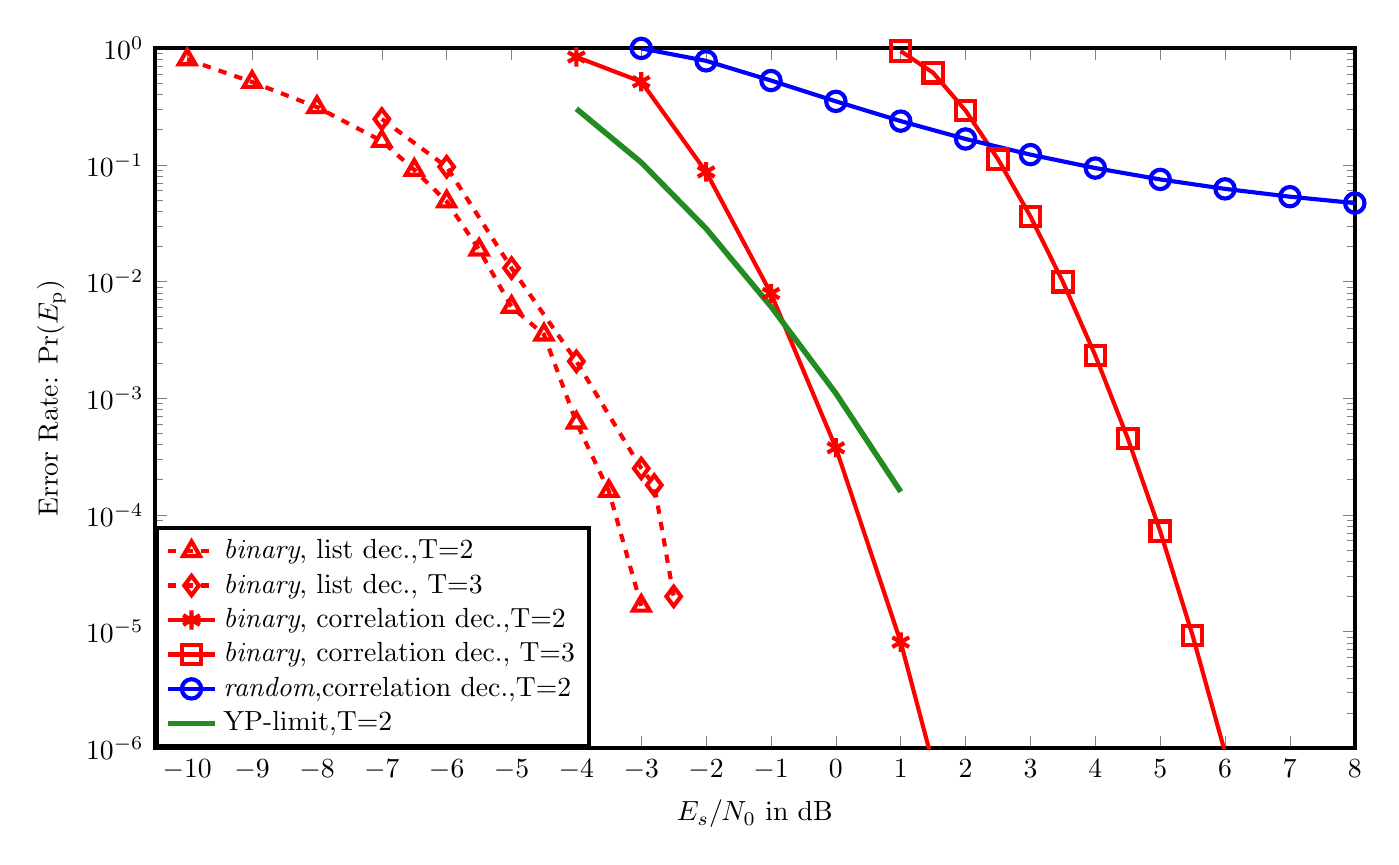
\begin{tikzpicture}

\begin{axis}[%
width=6in,
height=3.5in,
scale only axis,
xmin=-10.5,
xmax=8,
xtick={-10,-9,...,8},
xlabel={$E_s/N_0$ in dB},
ymode=log,
ymin=1e-6,
ymax=1,
ylabel={Error Rate: $\Pr(\mc{E}_{\mathrm{p}})$},
line width=1.5pt,
mark size=3.5pt,
legend style={at={(0,0)},anchor=south west,draw=black,fill=white,legend cell align=left}
]

\addplot [color=red,dashed,mark=triangle,mark options={solid}]
  table[row sep=crcr]{
  -10.00 8.000000e-01 \\
-9.00 5.128205e-01 \\
-8.00 3.125000e-01 \\
-7.00 1.600000e-01 \\
-6.50 9.049774e-02 \\
-6.00 4.842615e-02 \\
-5.50 1.876173e-02 \\
-5.00 6.064281e-03 \\
-4.50 3.506926e-03 \\
-4.00 6.165798e-04 \\
-3.5 1.60e-4\\
-3   1.66e-5\\
};
\addlegendentry{\emph{binary}, list dec.,T=2};

\addplot [color=red,dashed,mark=diamond,mark options={solid}]
  table[row sep=crcr]{
-7.00 2.469136e-01 \\
-6.00 9.615385e-02 \\
-5.00 1.302932e-02 \\
-4.00 2.067825e-03 \\
-3.00  2.50e-4\\
-2.8    1.80e-4\\
-2.50  2.00e-5\\
};
\addlegendentry{\emph{binary}, list dec., T=3};

%--------------Binary Correlation---------------------------------------
\addplot [color=red,solid,mark=asterisk]
  table[row sep=crcr]{-4	0.839938973915005\\
-3	0.515644197871796\\
-2	0.0869483964858722\\
-1	0.00788931487190525\\
0	0.000375462939704696\\
1	8.10369067605343e-06\\
2	6.47753143345753e-08\\
3	1.4828516192722e-10\\
4	7.03881397612349e-14\\
};
\addlegendentry{\emph{binary}, correlation dec.,T=2};


\addplot [color=red,solid,mark=square]
  table[row sep=crcr]{
1.00 9.441071e-01 \\
1.50 6.145469e-01 \\
2.00 2.916389e-01 \\
2.50 1.116871e-01 \\
3.00 3.606143e-02 \\
3.50 9.930853e-03 \\
4.00 2.319413e-03 \\
4.50 4.526161e-04 \\
5.00 7.231748e-05 \\
5.50 9.236722e-06 \\
6.00 9.177669e-07 \\
6.50 6.879983e-08 \\
7.00 3.759705e-09 \\
7.50 1.441054e-10 \\
8.00 3.710032e-12 \\
};
\addlegendentry{\emph{binary}, correlation dec., T=3};

%--------------Random Correlation---------------------------------------
\addplot [color=blue,solid,mark=o]
table[row sep=crcr]{
-3	0.995230206114719\\
-2	0.778551914311517\\
-1	0.527915283916314\\
0	0.350147600825551\\
1	0.237010766866583\\
2	0.166567660059161\\
3	0.122277177522\\
4	0.0937964411765719\\
5	0.0749838370997399\\
6	0.0622164196527422\\
7	0.0533299595443338\\
8	0.0470037470917604\\
9	0.0424113405143324\\
10	0.0390218393634084\\
11	0.0364852502123492\\
12	0.0345650780260551\\
13	0.0330978144887919\\
14	0.0319680291755858\\
15	0.0310926979824901\\
};
\addlegendentry{\emph{random},correlation dec.,T=2};

%-----------------------------------------------------------------
\addplot [color=ForestGreen,solid,line width=2pt]
table[row sep=crcr]{
-4  0.3022\\
-3	 0.1048\\
-2	 0.0284\\
-1	0.0061\\
0	0.0011\\
1 1.5778e-04\\
};
\addlegendentry{YP-limit,T=2};



\end{axis}
\end{tikzpicture}%}
\end{frame}


%%%%%%%%%%%----------------------------------------------------------------------------------%%%%%%%%%%%%%%%
\begin{frame}
\frametitle{Channel coding}
\begin{itemize}
\item \emph{``same-codebook"} scheme achieves GMAC capacity?
\item SC-LDPC (3,6), (3,9) codes for 2-user GMAC
\end{itemize}
\centering
\resizebox{0.55\textwidth}{!}{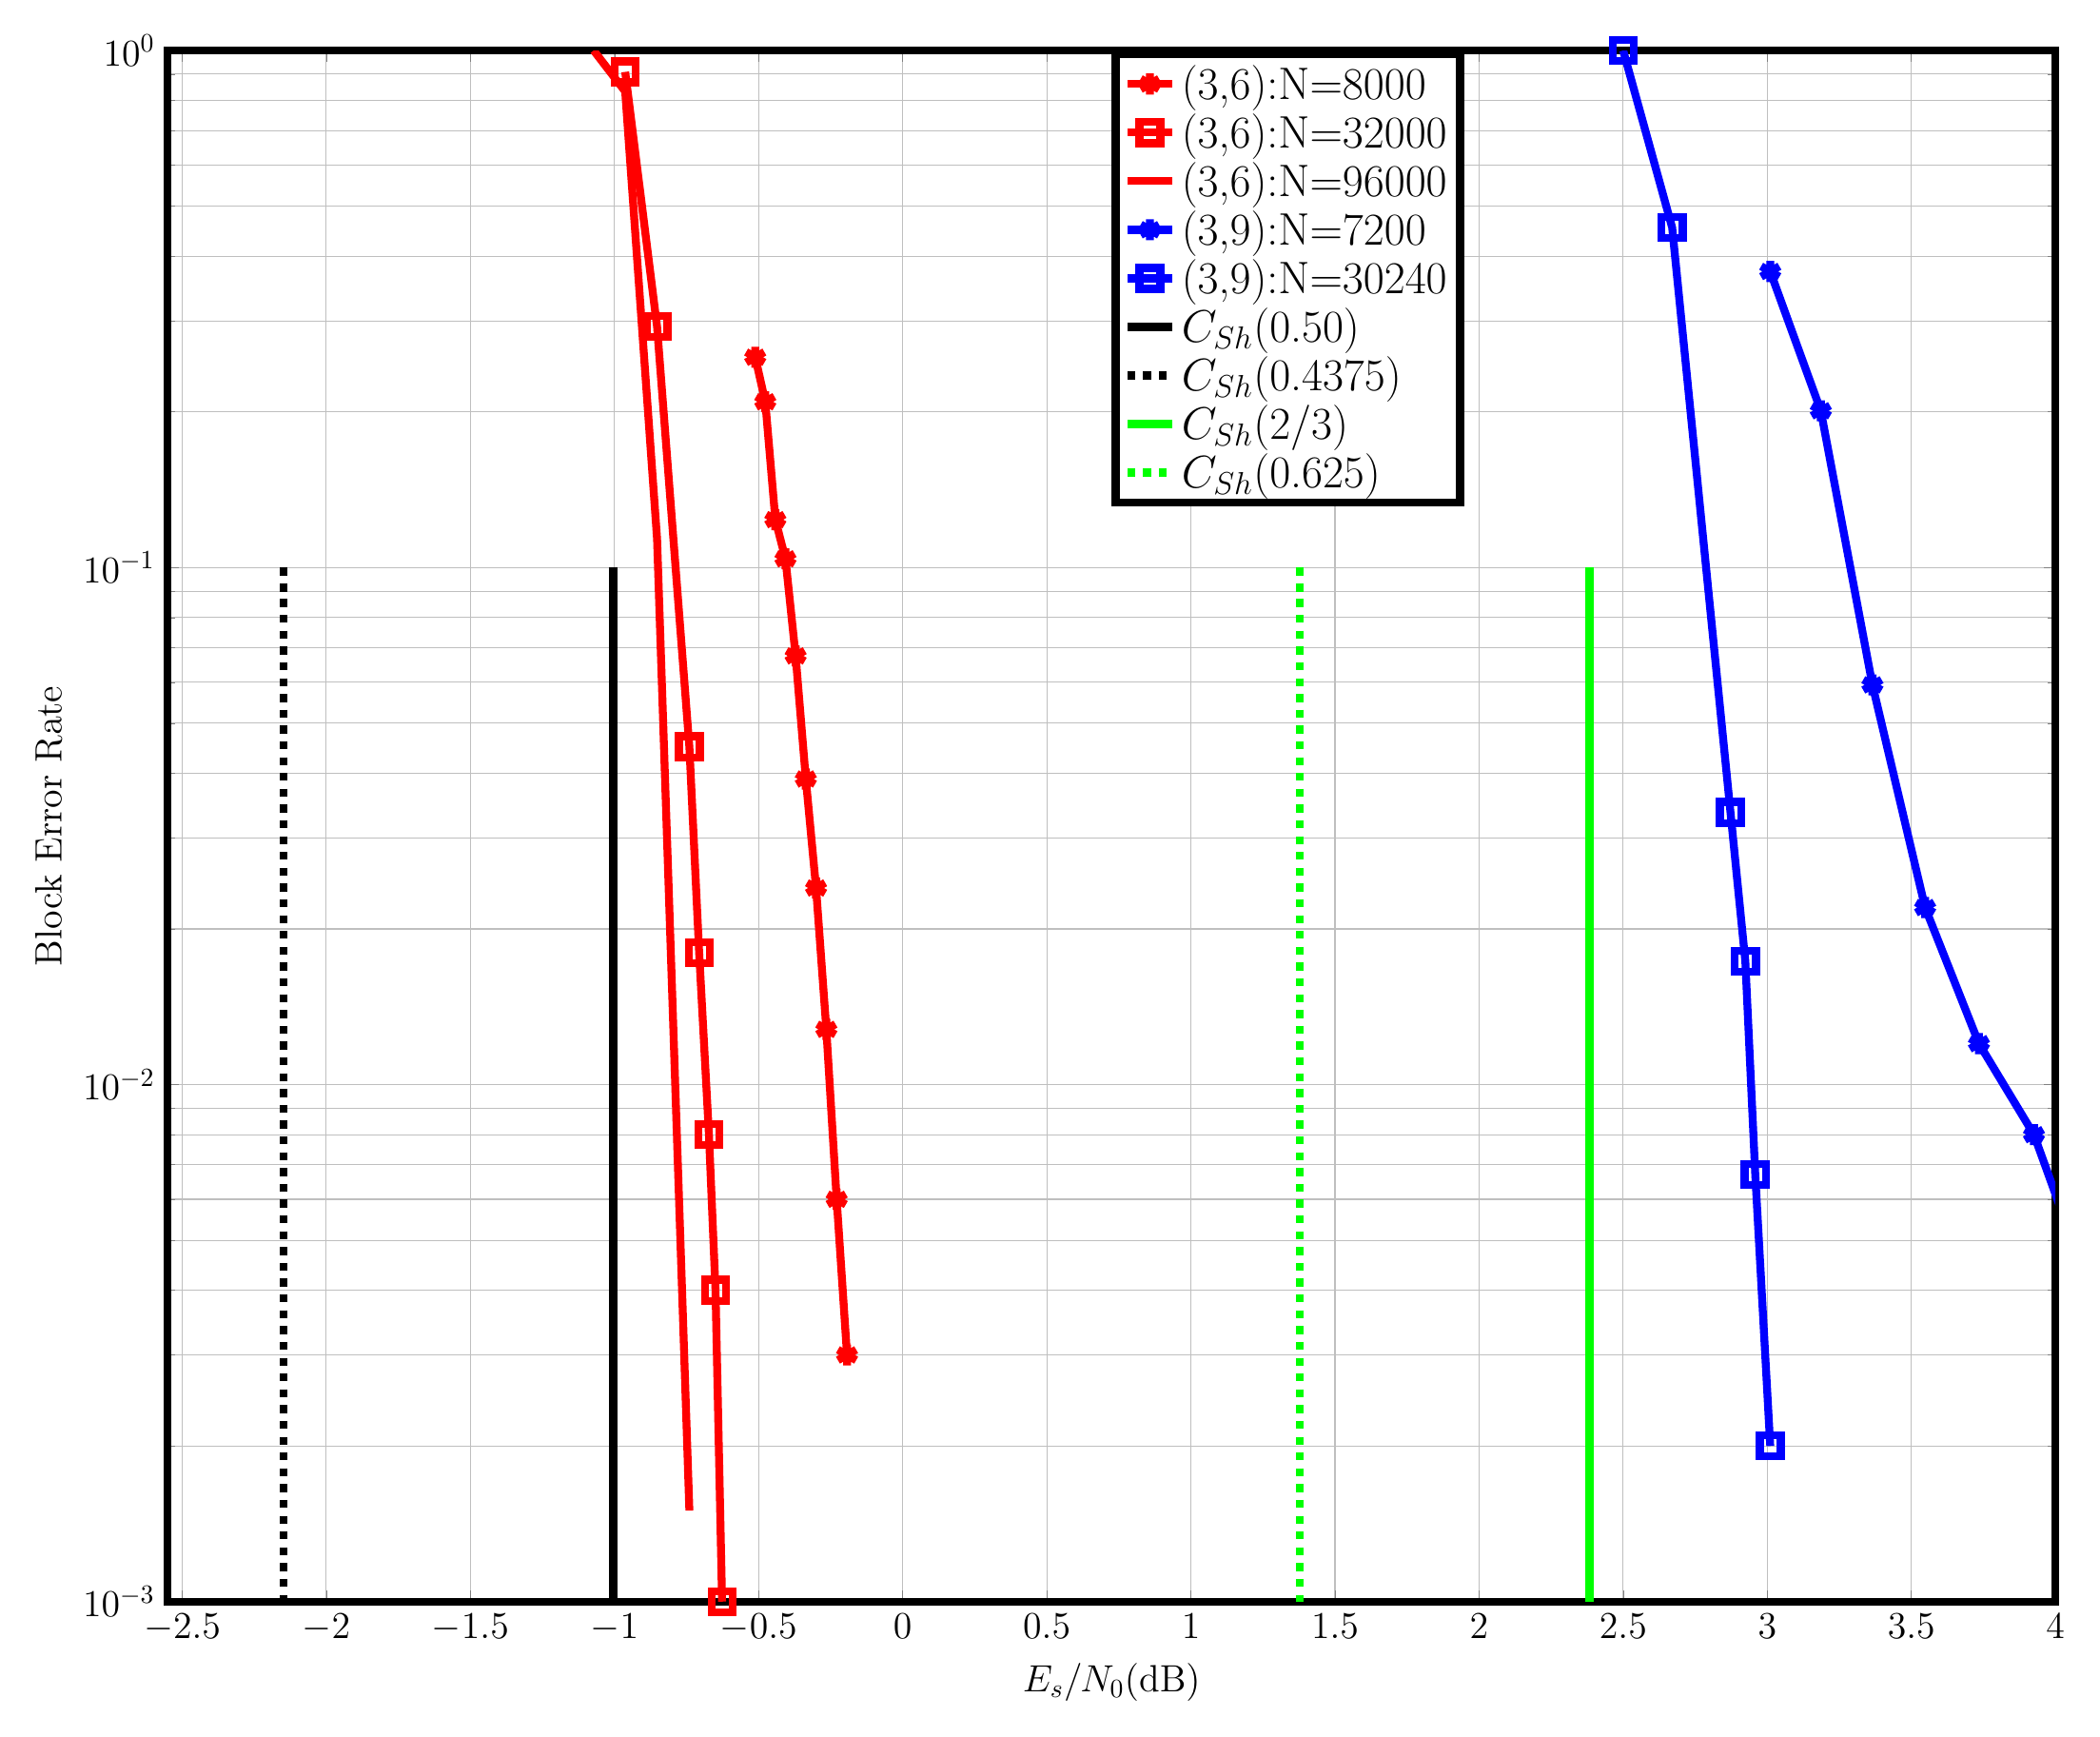
\begin{tikzpicture}
% The SC paramaters for the below set of plots are
% L=16
% w=3.
% So the true rate R is related to design rate R'(=1-dc/dv) as
% 1-R=(L+w-1)*(1-R')/L
\def\fsize{\Large}
\pgfplotsset{every y tick label/.append style={font=\Large}}
\pgfplotsset{every x tick label/.append style={font=\fsize}}

\begin{axis}[%
width=9.91942366579178in,
height=8.14846697287839in,
scale only axis,
xmin=-2.55,
xmax=4,
xtick = {-2.5,-2.0,...,4.5},
xlabel={\fsize{$E_s/N_0$(dB)}},
ylabel={\fsize{Block Error Rate}},
xmajorgrids,
ymode=log,
ymin=0.001,
ymax=1,
yminorticks=true,
ymajorgrids,
yminorgrids,
line width=3.0pt,
legend style={at={(0.5,1)},anchor=north west, draw=black,fill=white,legend cell align=left,font=\LARGE}
]

\addplot [color=red,solid,mark=asterisk,mark size=4.0]
  table[row sep=crcr]{-0.511525224473813	0.255102040816327\\
-0.476711992947787	0.209205020920502\\
-0.441758667557386	0.123762376237624\\
-0.406664116226376	0.103950103950104\\
-0.371427193100643	0.0674763832658569\\
-0.33604673832371	0.039\\
-0.300521577807649	0.024\\
-0.264850522999304	0.0127877237851662\\
-0.229032370641686	0.006\\
-0.193065902530428	0.003\\
};
\addlegendentry{(3,6):N=8000};


\addplot [color=red,solid,mark=square,mark size=4.0]%,mark options={solid}]
  table[row sep=crcr]{
   -0.9628    0.9091\\
   -0.8522    0.2924\\
   -0.7401    0.0450\\
   -0.7062    0.0180\\
   -0.6722    0.0080\\
   -0.6494    0.0040\\
   -0.6266    0.0010\\
 };
\addlegendentry{(3,6):N=32000};

\addplot [color=red,solid,mark=<,mark size=4.0]%,mark options={solid}]
  table[row sep=crcr]{
   -1.0721    1.0000\\
   -0.9628    0.8333\\
   -0.8522    0.1136\\
   -0.7401    0.0015\\
 };
\addlegendentry{(3,6):N=96000};


\addplot [color=blue,solid,mark=asterisk,mark size=4.0]
  table[row sep=crcr]{
   3.0103    0.3738\\
    3.1858    0.2010\\
    3.3649    0.0593\\
    3.5477    0.0220\\
    3.7345    0.0120\\
    3.9254    0.0080\\
    4.1206    0.0040\\
    4.3203    0.0020\\
};
\addlegendentry{(3,9):N=7200};

\addplot [color=blue,solid,mark=square,mark size=4.0]
  table[row sep=crcr]{
	2.50    1.0\\
	2.67   0.4545\\
    2.8724    0.0336\\
    2.9239    0.0173\\
    2.9583    0.0067\\
    3.0103    0.0020\\
};
\addlegendentry{(3,9):N=30240};



\addplot [color=black,solid]
  table[row sep=crcr]{
   -1.0041    0.1000\\
   -1.0041    0.0950\\
   -1.0041    0.0900\\
   -1.0041    0.0850\\
   -1.0041    0.0800\\
   -1.0041    0.0750\\
   -1.0041    0.0700\\
   -1.0041    0.0650\\
   -1.0041    0.0600\\
   -1.0041    0.0550\\
   -1.0041    0.0500\\
   -1.0041    0.0450\\
   -1.0041    0.0400\\
   -1.0041    0.0350\\
   -1.0041    0.0300\\
   -1.0041    0.0250\\
   -1.0041    0.0200\\
   -1.0041    0.0150\\
   -1.0041    0.0100\\
   -1.0041    0.0050\\
   -1.0041    0.0010\\
};
\addlegendentry{$C_{Sh}$(0.50)};

\addplot [color=black,dashed]
  table[row sep=crcr]{
   -2.1477    0.1000\\
   -2.1477    0.0950\\
   -2.1477    0.0900\\
   -2.1477    0.0850\\
   -2.1477    0.0800\\
   -2.1477    0.0750\\
   -2.1477    0.0700\\
   -2.1477    0.0650\\
   -2.1477    0.0600\\
   -2.1477    0.0550\\
   -2.1477    0.0500\\
   -2.1477    0.0450\\
   -2.1477    0.0400\\
   -2.1477    0.0350\\
   -2.1477    0.0300\\
   -2.1477    0.0250\\
   -2.1477    0.0200\\
   -2.1477    0.0150\\
   -2.1477    0.0100\\
   -2.1477    0.0050\\
   -2.1477    0.0010\\
   };
\addlegendentry{$C_{Sh}$(0.4375)};
   
   
   
   
\addplot [color=green,solid]
  table[row sep=crcr]{
    2.3835    0.1000\\
    2.3835    0.0950\\
    2.3835    0.0900\\
    2.3835    0.0850\\
    2.3835    0.0800\\
    2.3835    0.0750\\
    2.3835    0.0700\\
    2.3835    0.0650\\
    2.3835    0.0600\\
    2.3835    0.0550\\
    2.3835    0.0500\\
    2.3835    0.0450\\
    2.3835    0.0400\\
    2.3835    0.0350\\
    2.3835    0.0300\\
    2.3835    0.0250\\
    2.3835    0.0200\\
    2.3835    0.0150\\
    2.3835    0.0100\\
    2.3835    0.0050\\
    2.3835    0.0010\\
    };
\addlegendentry{$C_{Sh}$(2/3)};



\addplot [color=green,dashed]
  table[row sep=crcr]{
	1.3786    0.1000\\
    1.3786    0.0950\\
    1.3786    0.0900\\
    1.3786    0.0850\\
    1.3786    0.0800\\
    1.3786    0.0750\\
    1.3786    0.0700\\
    1.3786    0.0650\\
    1.3786    0.0600\\
    1.3786    0.0550\\
    1.3786    0.0500\\
    1.3786    0.0450\\
    1.3786    0.0400\\
    1.3786    0.0350\\
    1.3786    0.0300\\
    1.3786    0.0250\\
    1.3786    0.0200\\
    1.3786    0.0150\\
    1.3786    0.0100\\
    1.3786    0.0050\\
    1.3786    0.0010\\
        };
\addlegendentry{$C_{Sh}$(0.625)};


   
   
\end{axis}
\end{tikzpicture}%}
\end{frame}

%%%%%%%%%%%%----------------------------------------------------------------------------------%%%%%%%%%%%%%%%
\begin{frame}
\frametitle{Channel coding}
\begin{itemize}
\item $\Bc$ is fixed however $\#$ ch. uses for ch. coding, per slot, not fixed
\item necessitates construction of LDPC codes of arbitrary rates 
\item We use FBL ach. limit from [Polyanskiy-2017]
%\[
%P (\mc{E}_{\mathrm{c}})\leq h_{\text{FBL}}(N_{\mathrm{c}},2^{\Bc},T,P)\coleq \sum_{t=1}^{T} \min(p_t,q_t)+p_0,
%\]
\end{itemize}
\onslide<2->{
\vspace{2ex}
\centering
\footnotesize{Rate-1/4: LDPC (3,6) code constructed via PEG+ repeat twice}
\resizebox{0.5\textwidth}{!}{% This file was created by matlab2tikz v0.4.7 running on MATLAB 7.14.
% Copyright (c) 2008--2014, Nico Schlömer <nico.schloemer@gmail.com>
% All rights reserved.
% Minimal pgfplots version: 1.3
% 
% The latest updates can be retrieved from
%   http://www.mathworks.com/matlabcentral/fileexchange/22022-matlab2tikz
% where you can also make suggestions and rate matlab2tikz.
% 
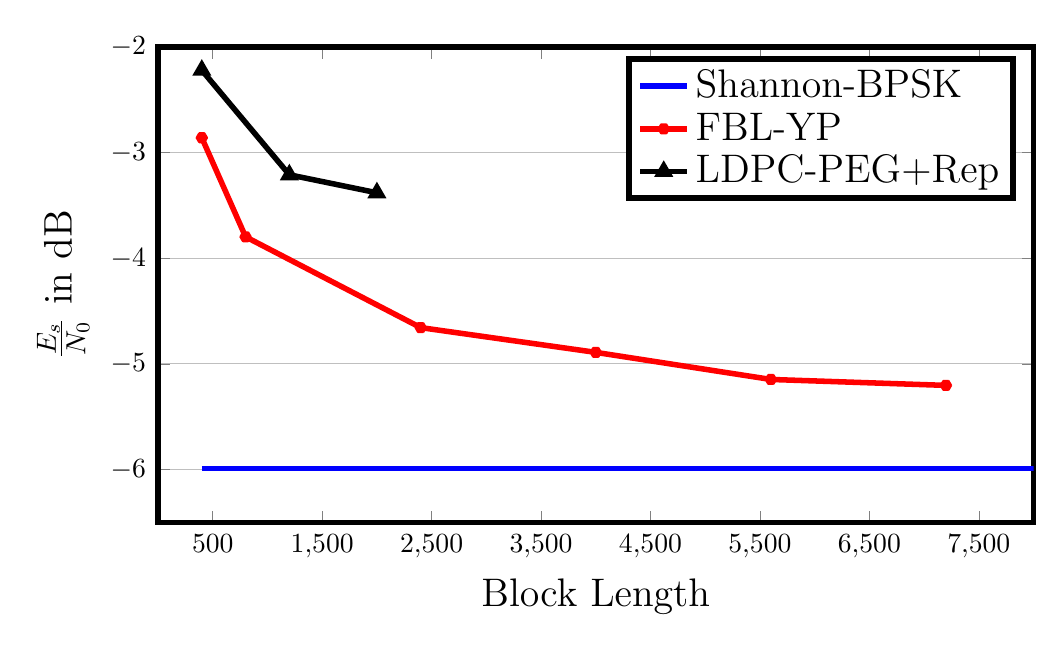
\begin{tikzpicture}
\def\fsize{\Large}

\begin{axis}[%
width=5in,
height=3in,
%scale only axis,
xmin=0,
xmax=8000,
xlabel={\fsize{Block Length}},
xtick={500,1500,...,7500},
ymin=-6.5,
ymax=-2,
ylabel={\fsize{$\frac{ E_s}{N_0}$ in dB}},
ymajorgrids,
line width=2pt,
%title={\fsize{FBL bounds comparison for Rate-1/4}},
legend style={draw=black,fill=white,legend cell align=left,font=\fsize}
]

\addplot [color=blue,solid]
  table[row sep=crcr]{
  400	-5.99\\
900	-5.99\\
1000	-5.99\\
1500	-5.99\\
2000	-5.99\\
2500	-5.99\\
3000	-5.99\\
3500	-5.99\\
4000	-5.99\\
4500	-5.99\\
5000	-5.99\\
5500	-5.99\\
6000	-5.99\\
6500	-5.99\\
7000	-5.99\\
7500	-5.99\\
8000	-5.99\\
};
\addlegendentry{Shannon-BPSK};

\addplot [color=red,solid,mark=asterisk,mark options={solid}]
  table[row sep=crcr]{
400	-2.8594\\
800	-3.7969\\
2400	-4.6562\\
4000	-4.8906\\
5600	-5.1469\\
7200	-5.2031\\
};
\addlegendentry{FBL-YP};

\addplot [color=black,solid,mark=triangle,mark options={solid}]
  table[row sep=crcr]{
  400	-2.22\\
1200	-3.21\\
2000	-3.38\\
};
\addlegendentry{LDPC-PEG+Rep};
\end{axis}

\end{tikzpicture}%}
}
\end{frame}
%%%%%%%%%%%%----------------------------------------------------------------------------------%%%%%%%%%%%%%%%
\begin{frame}\frametitle{Performance optimization}
$K\in[25:300], B=100, n=30,000$. For each $T\in\{2,4,5\}$
\begin{align*}
\frac{E_b}{N_0}&=\min_{\beta} \frac{(2-\beta)(N  P_{\text{slot}})}{2B}\\
\text{ ~~where }&\\
V&\coleq \arg\min_{V}~\Pr(\mc{E}'_{T\text{-peeling}}(K,V,T))\leq 0.04\\
P_p&\coleq \arg\min_{P}~ \Pr(\mc{E}_{\mathrm{p}})\leq \frac{0.01}{2V}\\
N&\coleq\left\lfloor \frac{n}{V}\right\rfloor\\
P_c&\coleq \arg\min_{P}~\Pr(\mc{E}_{\mathrm{c}} (N_c,B_\mathrm{c},T,P))\leq \frac{0.01}{2V}\\
P_{\text{slot}}&=\frac{N_p P_p+ N_c P_c}{N}
\end{align*}
\end{frame}

%%%%%%%%%%%%----------------------------------------------------------------------------------%%%%%%%%%%%%%%%
\begin{frame}
\centering
\resizebox{0.7\textwidth}{!}{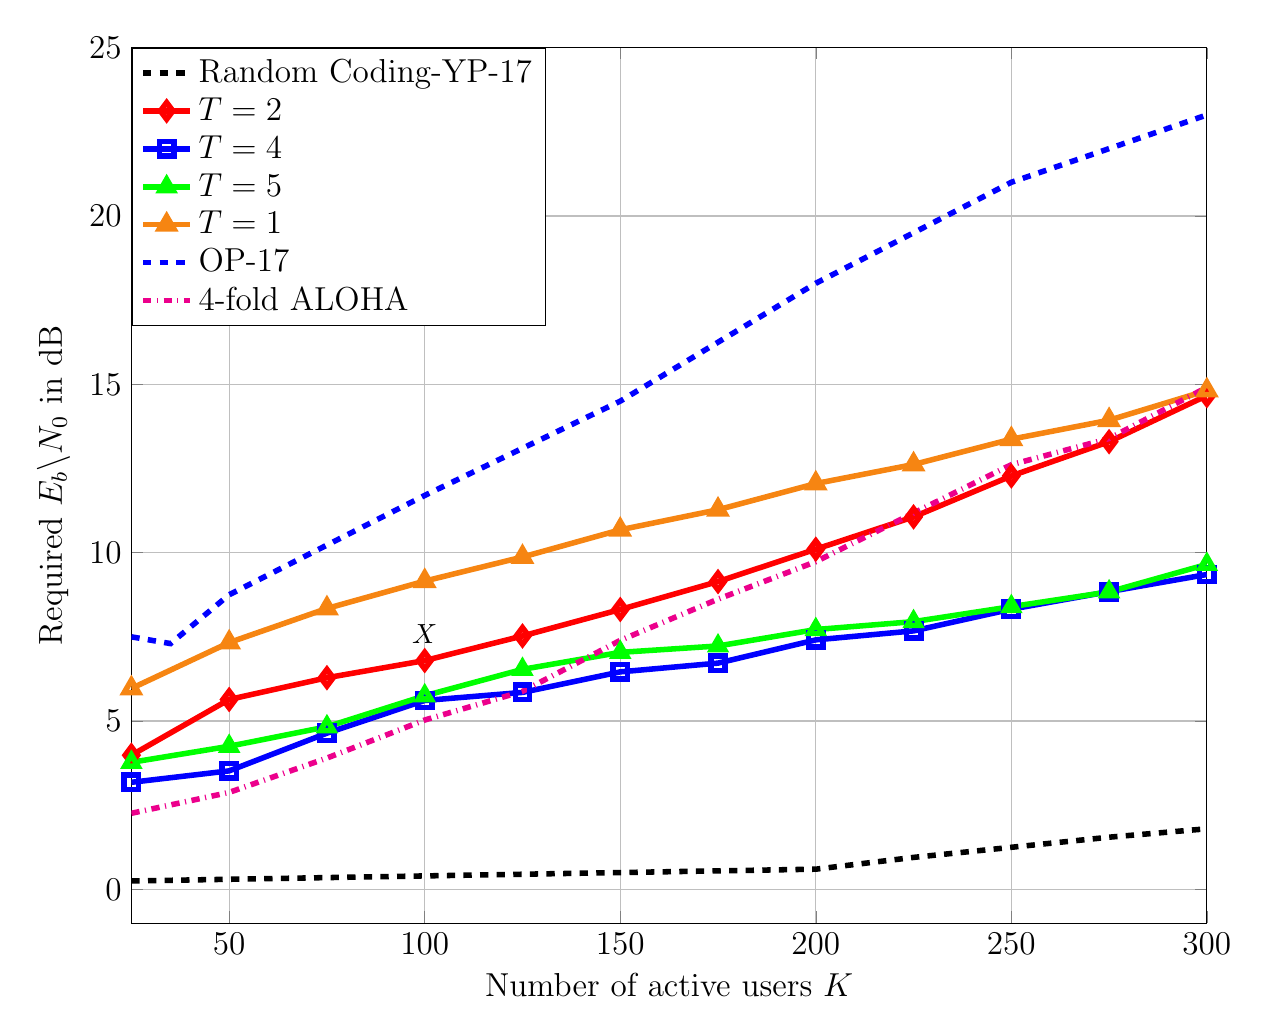
\begin{tikzpicture}
\def\fsize{\large}

\pgfplotsset{every y tick label/.append style={font=\fsize}}
\pgfplotsset{every x tick label/.append style={font=\fsize}}

\begin{axis}[%
width=6in,
height=5in,
xmin=25,
xmax=300,
xtick = {50,100,...,300},
xlabel={\fsize{Number of active users $K$}},
ylabel={\fsize{Required $E_b\backslash N_0$ in dB}},
xmajorgrids,
xminorgrids,
ymin=-1,
ymax=25,
ytick = {-5,0,...,30},
yminorticks=true,
ymajorgrids,
yminorgrids,
legend style={at={(0,1)},anchor=north west, draw=black,fill=white,legend cell align=left,font=\fsize}
]

\node[] at (axis cs: 100,7.5696) {$X$};

\addplot [color=black,solid,dashed, line width=2.0pt]
  table[row sep=crcr]{
  25     0.25\\
 50     0.3\\
 75     0.35\\
100     0.4\\
125     0.45\\
150     0.5\\
175    0.55\\
200  0.60\\
225 0.95\\
250 1.25\\
275 1.55\\
300 1.8\\
};
\addlegendentry{Random Coding-YP-17};

\addplot [color=red,solid,mark=diamond,mark size=3.0, line width=2.0pt]
  table[row sep=crcr]{
  25   3.9849  \\
  50   5.6396\\
  75   6.2855  \\
100  6.7952 \\
125  7.5262 \\
150  8.3122 \\
175  9.1418 \\
200  10.103 \\
225  11.062 \\
250  12.279 \\
275 13.296 \\
300 14.6648 \\
};
\addlegendentry{$T=2$};

\addplot [color=blue,solid,mark=square,mark size=2.6, line width=2.0pt]
  table[row sep=crcr]{
 25 3.18\\
 50 3.52\\
 75 4.64\\
100 5.61\\
125 5.85\\
150 6.46\\
175 6.72\\
200 7.41\\
 225 7.6772\\
 250 8.3217\\
 275 8.8428\\
 300 9.3520 \\
};
\addlegendentry{$T=4$};

%\addplot [color=blue,dotted, line width=2.0pt]
%  table[row sep=crcr]{
% 25 2.8815\\
% 50 3.2015\\
% 75 4.3960\\
%100 5.30\\
%125 5.5533\\
%150 6.1838\\
%175 6.4562\\
%200 7.1900\\
% 225 7.4664\\
% 250 8.1394\\
% 275 8.6810\\
% 300 9.2079 \\
%};
%\addlegendentry{$T=4$,ML-CS};

\addplot [color=green,mark=triangle,mark size=2.7, line width=2.0pt]
  table[row sep=crcr]{
 25 3.7732\\
 50 4.25\\
 75 4.8287\\
100 5.7503\\
125 6.5344\\
150 7.0391\\
175 7.2288\\
200 7.7171\\
 225 7.9514 \\
250 8.3968\\
275 8.8358\\
300  9.6524\\
};
\addlegendentry{$T=5$};

\addplot [color=BurntOrange,solid,mark=triangle,mark size=3.0, line width=2.0pt]
table[row sep=crcr]{
25 5.9675\\
50 7.33\\
75 8.3433\\
100 9.1555\\
125 9.8708\\
150 10.679\\
175 11.275\\
200 12.052 \\
225 12.61860 \\
250 13.3702 \\
275 13.934\\
300 14.816\\
 };
\addlegendentry{$T=1$}; %After Yury's correction



\addplot [color=blue,dashed, line width=2.0pt]
  table[row sep=crcr]{
  25   7.50 \\
   35   7.30 \\
  50   8.75 \\
  100 11.7 \\
  150 14.50\\
%175  6.7814 \\
200  18\\
%225  7.6838 \\
250  21\\
%275  8.4960 \\
300 23\\
};
\addlegendentry{OP-17};

\addplot [color=magenta,dash dot,line width=2.0pt]
  table[row sep=crcr]{
  25   2.26  \\
  50   2.88  \\
  75   3.90  \\
 100   5.03 \\
  125.0000    5.8798 \\
  150.0000    7.3954 \\
  175.0000    8.6199 \\
  200.0000    9.7328 \\
  225.0000   11.1761\\
  250.0000   12.6127\\
  275.0000   13.3907\\
  300.0000   14.9116\\
  };
\addlegendentry{4-fold ALOHA};

\end{axis}
\end{tikzpicture}}
\end{frame}

%%%%%%%%%%%%----------------------------------------------------------------------------------%%%%%%%%%%%%%%%
\begin{frame}{Conclusion}
\begin{itemize}  
  \item Proposed a practical coding scheme for the timely unsourced MAC problem
  \item Performance within $\approx 6$dB from the random coding ach. limit
  \item Same codebook schemes can perform optimally for GMAC
  \item Leverages the peeling decoder from coding theory  
\end{itemize}

\pause
Open Problems
\begin{itemize}
  \item A strict FBL lower bound for GMAC?
  \item Design of optimal matrices for the discussed $T$-sparse CS problem
\end{itemize}
\end{frame}

%\begin{frame}\frametitle{Tanner graph}
%\centering
%\resizebox{0.56\textwidth}{!}{\begin{tikzpicture}
\def\horzgap{7ex}; %Horizontal gap between nodes/levels
\def \gapVN{4ex}; %vertical gap between variable nodes
\def \gapCN{5ex}; %Horizontal gap between check nodes
\def\nodewidth{1.5ex};

\def \textoffs{1ex}; %Offset for writing text east of a node
%\def\nodewidthA{0.05in};
%\def \edgewidth{0.02in};
%\def\ext{0.2in};
`
\def \n{8};
\def\ldeg{2};
\def \m {4};
\def\rdeg{3};

\def\langle{40};%120 degrees/3
\def\langle{20};%120 degrees/6

\tikzstyle{check} = [rectangle, draw, line width=0.4pt, inner sep=0mm, minimum height=0.8*\nodewidth, minimum width=1.6*\nodewidth]%,rounded corners]
\tikzstyle{bit} = [circle, draw,line width=0.6pt, inner sep=0mm, minimum size=0.6*\nodewidth]

                          
\foreach \vn in {1,...,6}{
 \node[bit] (vn\vn) at (0,-\vn*\gapVN) {};
}


\foreach \cn in {1,...,4}{
\node[check] (cn\cn) at (\horzgap,-0.1*\gapCN-\cn*\gapCN) {};
}

\draw [decorate,decoration={brace,amplitude=1pt,mirror,raise=0.2pt},xshift=2*\nodewidth] (cn1.south east) -- (cn1.north east) node [black,midway,xshift=4ex] {\tiny $n/m$ ch. uses};

\path (cn2)++(0,-0.4*\gapCN) node () {\small{$\vdots$}};
\path (cn3.east)++(\textoffs,0) node ()[anchor=west] {\tiny{$\yv_j=\sum\limits_{i\in\mc{N}_j}\xv_i+\zv$}};

\draw (vn4.east)--(cn4.west);
\draw  (vn5.east)--(cn4.west);

\draw (vn2.east)--(cn3.west);
\draw (vn3.east)--(cn3.west);
\draw  (vn6.east)--(cn3.west);

\draw (vn1.east)--(cn2.west);
\draw (vn2.east)--(cn2.west);
\draw (vn5.east)--(cn2.west);

\draw (vn1.east)--(cn1.west);
\draw (vn3.east)--(cn1.west);
\draw (vn4.east)--(cn1.west);

\node[align=left] () at (0,-6.5*\gapVN){\tiny $K$ active users};
\node () at (\horzgap,-4.5*\gapCN){\tiny $m$ slots};
%\node[align=left] () at (1.2*\horzgap,-4.7*\gapCN){\tiny each $n/m$ channel uses};

\end{tikzpicture}}
%\pause
%\vspace{3ex}
%\begin{itemize}
%\item power constraint $\implies $ sparse Tanner graph 
%\end{itemize}

% Differences between the LDPC Tanner graph. We do not know the connections since which K users transmitted in which slots. Having an assigned coordinated coordination scheme kind of tells us something about the indetity/source.
%\end{frame}


%%%%%%%%%%%%----------------------------------------------------------------------------------%%%%%%%%%%%%%%%
%\begin{frame}\frametitle{Potential solution via peeling decoder}
%\begin{itemize}
%\item Joint decoding via successive interference cancellation: $\textbf{peeling}$ algorithm
%\onslide<2->{
% \item Challenges in implementing peeling:
%	\begin{itemize}
%	\item Decoding in presence of noise
%	\item Tx slots of users unknown at AP
%	\item Power constraint $\implies$ need efficiency in repetition pattern
%	}
%	\end{itemize}
%\end{itemize}
%
%\begin{columns}
%\column{0.5\textwidth}
%\onslide<3->{
%\begin{block}{Solution}
%Proposed design scheme involves solutions to the above challenges
%\end{block} 
%}
%\column{0.4\textwidth}
%\centering
%\resizebox{\textwidth}{!}{\begin{tikzpicture}
\def\horzgap{7ex}; %Horizontal gap between nodes/levels
\def \gapVN{4ex}; %vertical gap between variable nodes
\def \gapCN{5ex}; %Horizontal gap between check nodes
\def\nodewidth{1.5ex};

\def \textoffs{1ex}; %Offset for writing text east of a node
%\def\nodewidthA{0.05in};
%\def \edgewidth{0.02in};
%\def\ext{0.2in};
`
\def \n{8};
\def\ldeg{2};
\def \m {4};
\def\rdeg{3};

\def\langle{40};%120 degrees/3
\def\langle{20};%120 degrees/6

\tikzstyle{check} = [rectangle, draw, line width=0.4pt, inner sep=0mm, minimum height=0.8*\nodewidth, minimum width=1.6*\nodewidth]%,rounded corners]
\tikzstyle{bit} = [circle, draw,line width=0.6pt, inner sep=0mm, minimum size=0.6*\nodewidth]

                          
\foreach \vn in {1,...,6}{
 \node[bit] (vn\vn) at (0,-\vn*\gapVN) {};
}


\foreach \cn in {1,...,4}{
\node[check] (cn\cn) at (\horzgap,-0.1*\gapCN-\cn*\gapCN) {};
}

%\draw [decorate,decoration={brace,amplitude=1pt,mirror,raise=0.2pt},xshift=2*\nodewidth] (cn1.south east) -- (cn1.north east) node [black,midway,xshift=4ex] {\tiny $n/m$ ch. uses};

\path (cn2)++(0,-0.4*\gapCN) node () {\small{$\vdots$}};
\path (cn3.east)++(0.8*\textoffs,0) node ()[anchor=west] {\tiny{$\yv_j=\sum\limits_{i\in\mc{N}_j}\xv_i+\zv$}};

\draw (vn4.east)--(cn4.west);
\draw  (vn5.east)--(cn4.west);

\draw (vn2.east)--(cn3.west);
\draw (vn3.east)--(cn3.west);
\draw  (vn6.east)--(cn3.west);

\draw (vn1.east)--(cn2.west);
\draw (vn2.east)--(cn2.west);
\draw (vn5.east)--(cn2.west);

\draw (vn1.east)--(cn1.west);
\draw (vn3.east)--(cn1.west);
\draw (vn4.east)--(cn1.west);

\node[align=left] () at (0,-6.5*\gapVN){\tiny $K$ active users};
\node () at (\horzgap,-4.5*\gapCN){\tiny $m$ slots};
%\node[align=left] () at (1.2*\horzgap,-4.7*\gapCN){\tiny each $n/m$ channel uses};

\end{tikzpicture}}
%\end{columns}
%\end{frame}
